%
% Niniejszy plik stanowi przykład formatowania pracy magisterskiej na
% Wydziale MIM UW.  Szkielet użytych poleceñ można wykorzystywać do
% woli, np. formatujac wlasna prace.
%
% Zawartosc merytoryczna stanowi oryginalnosiagniecie
% naukowosciowe Marcina Wolinskiego.  Wszelkie prawa zastrzeżone.
%
% Copyright (c) 2001 by Marcin Woliñski <M.Wolinski@gust.org.pl>
% Poprawki spowodowane zmianami przepisów - Marcin Szczuka, 1.10.2004
% Poprawki spowodowane zmianami przepisow i ujednolicenie 
% - Seweryn Karłowicz, 05.05.2006
% dodaj opcję [licencjacka] dla pracy licencjackiej
\documentclass{pracamgr}

\usepackage{polski}

%Jesli uzywasz kodowania polskich znakow ISO-8859-2 nastepna linia powinna byc 
%odkomentowana
\usepackage[latin2]{inputenc}
%Jesli uzywasz kodowania polskich znakow CP-1250 to ta linia powinna byc 
%odkomentowana
%\usepackage[cp1250]{inputenc}
\usepackage{hyperref}
\usepackage{graphicx}
\usepackage{epstopdf}
\usepackage{listings}
\lstset{ %
language=C++,                % the language of the code
numbers=left,
frame=single,
showstringspaces=false,
inputencoding=utf8,
extendedchars=\true,
literate= {ą}{{\k{a}}}1
	  {Ą}{{\k{A}}}1
	  {ę}{{\k{e}}}1
	  {Ę}{{\k{E}}}1
	  {ó}{{\'o}}1
	  {Ó}{{\'O}}1
	  {ś}{{\'s}}1
	  {Ś}{{\'S}}1
	  {ł}{{\l{}}}1
	  {Ł}{{\L{}}}1
	  {ż}{{\.z}}1
	  {Ż}{{\.Z}}1
	  {ź}{{\'z}}1
	  {Ź}{{\'Z}}1
	  {ć}{{\'c}}1
	  {Ć}{{\'C}}1
	  {ś}{{\'n}}1
	  {ś}{{\'N}}1
}

\usepackage{float}
\floatstyle{boxed} 
\restylefloat{figure}

\newcommand{\feval}{\texttt{eval}}
\newcommand{\dexp}{\texttt{deferred\_expr}}
\newcommand{\emgr}{\texttt{evaluation\_mgr}}
\newcommand{\dval}{\texttt{deferred\_value}}


\author{Paweł Tryfon}

\nralbumu{248444}

\title{Parallel -- biblioteka do równoległego obliczania wyrażeń w języku C++}

\tytulang{A library for parallel expression evaluation in C++}

%kierunek: Matematyka, Informatyka, ...
\kierunek{Informatyka}

% Praca wykonana pod kierunkiem:
% (podać tytuł/stopień imię i nazwisko opiekuna
% Instytut
% ew. Wydział ew. Uczelnia (jeżeli nie MIM UW))
\opiekun{dra Marcina Benke\\
  Zakład Logiki Stosowanej
  }

% miesiąc i~rok:
\date{Maj 2011}

%Podać dziedzinę wg klasyfikacji Socrates-Erasmus:
\dziedzina{ 
%11.0 Matematyka, Informatyka:\\ 
%11.1 Matematyka\\ 
%11.2 Statystyka\\ 
11.3 Informatyka\\ 
%11.4 Sztuczna inteligencja\\ 
%11.5 Nauki aktuarialne\\
%11.9 Inne nauki matematyczne i informatyczne
}

%Klasyfikacja tematyczna wedlug AMS (matematyka) lub ACM (informatyka)
\klasyfikacja{D. Software\\
  D.3. Programming languages\\
  D.3.3. Language Constructs and Features\\
  Subject: Concurrent Programming Constructs}

% Słowa kluczowe:
\keywords{obliczenia równoległe, C++, wielowątkowość, leniwe wyliczanie, programowanie generyczne}

% Tu jest dobre miejsce na Twoje własne makra i~środowiska:
%\newtheorem{defi}{Definicja}[section]

% koniec definicji

\begin{document}
\maketitle

%tu idzie streszczenie na strone poczatkowa
\begin{abstract}
  Obecne architektury pozwalają na przyspieszanie działania programów dzięki ich wykonywaniu jednocześnie na kilku procesorach.
  Jednakże skorzystanie z tej możliwości przedstawia istotną trudność dla programistów, gdyż programy wielowątkowe w swojej strukturze bardzo różnią się od programów sekwencyjnych.
  Projektowanie i implementacja programów wykorzystujących współbieżność jest znacznie bardziej czasochłonna oraz wymaga wyższych kwalifikacji.
  Niniejsza praca podejmuje próbę stworzenia biblioteki, która ułatwiłaby zadanie programowania programów wielowątkowych.  
  Głównym priorytetem byłu umożliwienie programiście zrównoleglania obliczeń w zwięzły, zrozumiały i prosty sposób.    
  Obecnie nie istnieje w języku C++ żadna biblioteka oferująca taką funcjonalność.
  Praca przedstawia model prowadzenia obliczeń równoległych w języku C++ oraz prezentuje proponowaną implementację.
  W pracy zostały szczegółowo opisane problemy, które zostały rozwiązane podczas projektowania biblioteki, 
  takie jak: mechanizm przekazywania wyrażeń do wyliczenia równoległego, sposób prowadzenia równoległych obliczeń, 
  sposób zwracania wyników obliczeń oraz metody zapobiegania problemom związanym z prowadzeniem równoległych obliczeń.
\end{abstract}

\tableofcontents
%\listoffigures
%\listoftables


\chapter*{Wprowadzenie}
\addcontentsline{toc}{chapter}{Wprowadzenie}

  R�wnoleg�e prowadzenie oblicze� nie jest w informatyce tematem nowym, gdy� liczy sobie ju� ponad 50 lat\cite{parhist}.
  Trudno jednak�e wskaza� konkretny punkt lub prac�, kt�re zapocz�tkowa�y ten kierunek rozwoju informatyki, ale niew�tpliwie do jego pionier�w nale�eli tak znani naukowcy jak
  Amdahl (prawo Amdahla), Flynn (klasyfikacja Flynna), Dijkstra (problem sekcji krytycznych oraz semafory) czy Petri (sieci Petriego).
  
  Zr�wnoleglanie oblicze� jest jednym ze sposob�w przyspieszania wydajno�ci system�w komputerowych.
  Metoda ta nabra�a ostatnio szczeg�lnego znaczenia, poniewa� rozw�j technologii mikroprocesorowej dotar� do takiego momentu, �e przyspieszanie pojedy�czej jednostki obliczeniowej sta�o si� trudne i w zwi�zku z tym nieop�acalne.
  Ze wzgl�du na to obecnie kierunek rozwoju wyznaczany jest przez r�wnoleg�o��, to znaczy umieszczanie w procesorach komputer�w wielu uk�ad�w wykonuj�cych obliczenia r�wnolegle w jednym czasie.
  Takie rozwi�zanie pozwala teoretycznie na uzyskanie przyspieszenia wprost proporcjonalnego do liczby uk�ad�w umieszczonych w procesorze.
  Aby uzyska� wspomniany wzrost wydajno�ci, programy wykonywane na takim procesorze powinny by� w stanie wykorzysta� mo�liwo�ci procesor�w wielordzeniowych.
  
  Jednak�e, pomimo d�ugo rozwijanej teorii oraz narz�dzi wspieraj�cych, programowanie r�wnoleg�e wci�� pozostaje bardzo trudne do zastosowania w praktyce.
  Dzieje si� tak, poniewa� wykorzystanie kilku w�tk�w wykonania programu, drastycznie zwi�ksza z�o�ono�� pracy programistycznej.
  Programista, aby napisa� program wsp�bie�ny (\cite{barney}) musi w pierwszej kolejno�ci zidentyfikowa� fragmenty oblicze�, kt�re mog� zosta� zr�wnoleglone.
  Nast�pnie powinien zaprojektowa� spos�b, w jaki poszczeg�lne w�tki wykonania si� ze sob� komunikuj� i w jaki s� synchronizowane.
  W celu zapewnienia efektywno�ci programu programista powinien uwzgl�dni� w projekcie r�wnie� balansowanie rozk�adu pracy pomiedzy poszczeg�lne w�tki wykonania.
  
  Programist� w zmaganiach z pisaniem program�w wsp�bie�nych wspieraj� r�norodne narz�dzia, j�zyki programowania specjalnie zaprojektowane do oblicze� r�wnoleg�ych, takie jak Ada, 
  lub biblioteki oferuj�ce wykonywanie oblicze� r�wnoleg�ych w j�zykach natywnie sekwencyjnych.
  Pierwsze wywi�zuj� si� zazwyczaj dobrze ze swojego zadania, gdy� s� dedykowane do programowania r�wnoleg�ego, lecz nie s� popularne w zastosowaniach praktycznych.
  Wi�kszym problemem jest korzystanie z drugiego typu narz�dzi, poniewa� j�zyk sekwencyjny cz�sto nie pozwala na zaprojektowanie biblioteki mog�cej konkurowa� prostot� i intuicyjno�ci� z j�zykiem do programowania r�wnoleg�ego.
  W praktyce potrzeba skorzystania z bibliotek dla j�zyk�w sekwencyjnych wyst�puje zdecydowanie cz�ciej, poniewa� j�zyki sekwencyjne s� znacznie szerzej stosowane.
  Niniejsza praca podejmuje pr�b� stworzenia biblioteki Parallel dla j�zyka C++ umo�liwiaj�cej r�wnoleg�e prowadzenie oblicze�.
  Nadrz�dnymi priorytetami podczas projektowania biblioteki by�o zapewnienie �atwo�ci pisania program�w r�wnoleg�ych z jednoczesnym pozostawieniem pe�nej kontroli nad wykonaniem programu w r�kach programisty. 
  Dzi�ki temu mia�y zosta� osi�gni�te dwa g��wne cele projektowania biblioteki: zwi�kszenie produktywno�ci programisty oraz zwi�kszenie szybko�ci dzia�ania program�w (przyspieszonych przez wykorzystanie r�wnoleg�o�ci).
  
  Biblioteka Parallel pozwala na zr�wnoleglanie oblicze� w spos�b, kt�ry nie ingeruje znacz�co w struktur� kodu.
  W celu skorzystania z biblioteki wystarczy przekaza� nieznacznie zmodyfikowane wyra�enie zgodne ze specyfikacj� biblioteki Parallel do funkcji bibliotecznej \verb|eval|, 
  co spowoduje przekazanie tego wyra�enia do wyliczenia przez aparat wykonawczy biblioteki Parallel, a nast�pnie zwr�cenie wyliczonej warto�ci.
  Najlepiej obja�ni to przyk�ad wykorzystania biblioteki.
  Pos�u�� si� w tym celu definicj� funkcji obliczaj�cej n-t� liczb� ci�gu Fibonacciego.
  Standardowo w j�zyku C++ kod tej funkcji wygl�da nast�puj�co:
  \begin{lstlisting}
  unsigned fibo(unsigned n)
  {
    if (n == 0)
      return 0;
    else if (n == 1)
      return 1;
    else
      return fibo(n-1) + fibo(n-2);
  }
  \end{lstlisting}
  Natomiast w przypadku wykorzystania biblioteki Parallel przyjmie on nast�puj�c� posta�:
  \begin{lstlisting}
  #include <parallel.h>
   
  unsigned fibo(unsigned n)
  {
    if (n == 0)
      return 0;
    else if (n == 1)
      return 1;
    else
      return parallel::eval(parallel::lazyf(fibo, n-1)) + fibo(n-2);
  }
  \end{lstlisting}
  
  Ten przyk�ad obrauje, w jaki spos�b mo�na wykorzysta� bibliotek� Parallel do zr�wnoleglenia oblicze� w podej�ciu ``dziel i zwyci�aj'', polegaj�cym na dzieleniu problemu na kilka cz�ci, z kt�rych ka�da jest obliczana r�wnolegle,
  Ko�cowy rezultat jest obliczany na podstawie wynik�w uzyskanych dla poszczeg�lnych podproblem�w.
  W tym przypadku zr�wnoleglenie b�dzie polega�o na tym, �e kod g��wny programu zleci r�wnoleg�e obliczenie wyra�enia \verb|fibo(n-1)| bibliotece Parallel i nie czekaj�c na wynik przejdzie do nast�pnej instrukcji,
  czyli obliczenia \verb|fibo(n-2)|. Po obliczaniu \verb|fibo(n-1)| i \verb|fibo(n-2)|, zostanie obliczona suma obu warto�ci i zwr�cona jako wynik \verb|fibo(n)|.
  Funkcja \feval z przestrzeni nazw \verb|parallel| s�u�y do r�wnoleg�ej ewaluacji wyra�e�, a funkcja \verb|lazyf| oznacza wykorzystywana jest do wywo�ania funkcji podanej jako pierwszy argument z parametrami podanymi jako kolejne argumenty \verb|lazyf|.
  Sk�adnia s�u��ca do korzystania z biblioteki Parallel zostanie dok�adniej opisana w dalszej cz�ci pracy.
  
  Pierwszy rozdzia� pracy opisuje koncepcj� biblioteki, g��wne zasady jej dzia�ania oraz por�wnuje projektowane rozwi�zanie do istniej�ch ju� rozwi�za�.
  Drugi rozdzia� traktuje o sposobie implementacji biblioteki.
  W trzecim rozdziale zosta�y przedstawione metody oraz wyniki ewaluacji biblioteki.
  Rozdzia� ostatni nakre�la mo�liwo�ci dalszego rozwoju biblioteki.

\newpage
\section*{Definicje poj�� i skr�t�w}
\begin{tabular}{ | l | p{0.75\textwidth} |}
  \hline\
  \textbf{Poj�cie} & \textbf{Definicja} \\ \hline
  API & Interfejs programowania aplikacji (z ang. Application Programming Interface) w kontek�cie bibliotek programistycznych jest opisem zestawu typ�w i funkcji, kt�re dana biblioteka udost�pnia. \\ \hline
  AST & Abstrakcyjne Drzewo Syntaktyczne (z ang. Abstract Syntax Tree) jest drzewem reprezentuj�cym struktur� kodu �r�d�owego w pewnym j�zyku programowania.\\ \hline
  Gorliwa semantyka & Semantyka, w kt�rej wyra�enia s� obliczane w miejscu pojawienia si� w programie. Przeciwie�stwem jest semantyka leniwa, w kt�rej wyra�enia obliczane s� tam, gdzie jest potrzebny ich wynik. \\ \hline
  Idempotentno�� & W�asno�� pewnej operacji, kt�ra pozwala na wielokrotne jej stosowanie bez zmiany wyniku. \\ \hline
  Idiom C++ & Konstrukcja j�zyka C++, kt�ra cz�sto pojawia si� w kodzie lub projektach do�wiadczonych programist�w C++. Stosowanie jej uwa�ane jest za dobr� praktyk�.\\  \hline

\end{tabular} 


\chapter{Koncepcja biblioteki}\label{r:koncepcja}

  W tym rozdziale zostan� przedstawione g��wne za�o�enia oraz szkic projektu biblioteki Parallel. 
  Ponadto biblioteka Parallel zostanie zestawiona z istniej�cymi bibliotekami do programowania r�wnoleg�ego w celu pokazania r�nic i uzasadnienia potrzeby stworzenia nowej biblioteki.

\section{Cele biblioteki}\label{s:cele}

  Tworzeniu biblioteki Parallel przy�wieca�y jasno sprecyzowane cele, kt�rych ide� przewodni� by�o u�atwienie wykorzystywania oblicze� r�wnoleg�ych w programach.
  Wymienionym poni�ej celom by�o podporz�dkowane projektowanie API i implementacja biblioteki.

\subsection{Wysoka efektywno��}

  Jednym z g��wnych powod�w stosowania zr�wnoleglania oblicze� jest przyspieszanie ich wykonania. 
  Zatem sama biblioteka do zr�wnoleglania powinna dzia�a� szybko.
  Niedopuszczaln� by�aby sytuacja, gdyby program wsp�bie�ny wykonywa� si� wolniej ni� jego sekwencyjny odpowiednik.
  Biblioteka Parallel b�dzie bibliotek� og�lnego zastosowania, przy pomocy, kt�rej b�dzie mo�liwe prowadzenie dowolnych oblicze�.
  W zwi�zku z tym, nie ma mo�liwo�ci zoptymalizowania biblioteki pod k�tem prowadzenia jednego z g�ry znanego typu oblicze�.
  Dlatego, opr�cz szybkiego dzia�ania mechanizm�w wbudowanych w bibliotek�, niezb�dne jest pozwolenie programi�cie na podejmowanie decyzji o takim prowadzeniu oblicze�, 
  �e ich wykonanie przy u�yciu biblioteki Parallel b�dzie efektywne.
  Kluczow� rol� odgrywa odpowiedni podzia� zada� przez programist�.
  
\subsection{Zwi�kszenie produktywno�ci programisty}

  Problem z produktywno�ci� programisty w przypadku pisania program�w r�wnoleg�ych polega na tym, �e takie programy s� trude do napisania, wi�c wymagaj� znacznych nak�ad�w pracy programist�w.
  Zr�wnoleglenie cho�by niewielkiego fragmentu programu wymaga znacznie wi�cej czasu ni� napisanie jego sekwencyjnego odpowiednika.
  By� mo�e dlatego obliczenia r�wnoleg�e wykorzystywane s� wy��cznie wtedy, gdy ju� nie ma innego sposobu osi�gni�cia niezb�dnego minimum wydajno�ci programu.
  Biblioteka Parallel celuje w zmian� tego stanu rzeczy poprzez wprowadzenie modelu programowania r�wnoleg�ego, kt�ry b�dzie tak intuicyjny jak programowanie sekwencyjne.
  Dzi�ki temu napisanie kodu, kt�ry dzia�a wsp�bie�nie, b�dzie w wielu przypadkach prawie tak samo szybkie jak kodu sekwencyjnego, co pozwoli�oby uzyska� programistom szybsze programy przy zbli�onej produktywno�ci ich pracy.

\subsection{Czytelno�� kodu}

  Tym, co najbardziej utrudnia zrozumienie program�w wsp�bie�nych jest konieczno�� zrozumienia zale�no�ci pomi�dzy odr�bnymi r�wnolegle dzia�aj�cymi cz�ciami programu.
  Zazwyczaj te zale�no�ci dotycz� miejsc w kodzie, kt�re s� od siebie stosunkowo odleg�e.
  Mnogo�� niejawnych zale�no�ci i przeplot�w wykona� programu sprawiaj�, �e nawet pozornie proste operacje s� trudne do poprawnego zaprogramowania, a przyczyny ewentualnych b��d�w s� bardzo trudne do zidentyfikowania.
  Jednym z bardziej wymownych przyk�ad�w popieraj�cych to stwierdzenie jest problem implementacji semafora uog�lnionego przy pomocy semafor�w binarnych \cite{gensem}, 
  kt�rego b��dne rozwi�zania pojawia�y si� w publikacjach naukowych i nawet przez kilka lat by�y uwa�ane za poprawne.
  St�d celem, kt�ry zosta� postawiony przed bibliotek� Parallel by�o stworzenie takiego modelu oblicze�, w kt�rym obliczenia r�wnoleg�e prowadzone by�yby w spos�b czytelny.
  Oznacza to, i� miejsca wykorzystania r�wnoleg�o�ci powinny by� wyra�nie widoczne i �atwe do odnalezienia, a sam zapis nie powinnien komplikowa� kodu.
  Najwa�niejsze jest to, �e struktura programu napisanego przy pomocy biblioteki Parallel nie powinna istotnie r�ni� si� od struktury programu sekwencyjnego.
  Pozwoli to na uzyskanie kodu, kt�ry b�dzie znacznie �atwiej zrozumie�.

\subsection{Transparencja}

  Biblioteka Parallel powinna udost�pnia� programi�cie wgl�d w to, w jaki spos�b obliczenia r�wnoleg�e b�d� prowadzone.
  Dzi�ki temu programista b�dzie m�g� uwzgl�dni� podczas programowania specyfik� biblioteki.
  Mi�dzy innymi b�dzie m�g� dostosowa� wielko�� zlecanych fragment�w oblicze� (ziarnisto�� oblicze�), tak aby zmaksymalizowa� wydajno�� programu.
  
\subsection{Abstrakcja}

  Abstrakcja ukrywa niepotrzebne szczeg�y implementacji przed programist�, co pozwala na zwi�kszenie jego produktywno�ci.
  Biblioteka powinna ofertowa� proste og�lne API, tak aby programista m�g�, po zapoznaniu si� z funkcjami oferowanymi przez bibliotek�, w kr�tkim czasie przyst�pi� do korzystania z Parallel.

\subsection{Ograniczenie konieczno�ci korzystania z mechanizm�w komunikacji i synchronizacji proces�w r�wnoleg�ych}

  Projektowawnie komunikacji i synchronizacji w programach wsp�bie�nych jest czym�, co decyduje o fakcie, �e programowanie r�wnoleg�e jest tak trudnym zadaniem.
  Celem biblioteki Parallel jest zdj�cie w znacznym stopniu tego obci��enia z programisty.
  Komunikacja pomi�dzy r�nymi w�tkami wykonania b�dzie koordynowana przez bibliotek�.
  Biblioteka nie mo�e wyr�czy� jednak programisty we wszystkim, ochrona sp�jno�ci struktur danych programu pozostanie w r�kach programisty.
  
\subsection{Przenaszalno��}
  
  Jest to bardzo istotna cecha biblioteki, dzi�ki kt�rej kod pisany przy u�yciu biblioteki Parallel b�dzie m�g� by� kompilowany i wykonywany na dowolnych platformach.
  Zostanie to osi�gni�te dzi�ki zaprogramowaniu biblioteki w pe�nej zgodno�ci z przysz�ym standardem j�zyka C++ (standard C++0x).
  U�ycie nowego standardu jest niezb�dne ze wzgl�du na zaawansowane konstrukcje j�zykowe potrzebne do zaprogramowania biblioteki Parallel.
  Konsekwencj� tego b�dzie niezgodno�� biblioteki z wcze�niejszymi standardami j�zyka C++, ale umo�liwi stworzenie lepszego, bardziej czytelnego kodu biblioteki przy u�yciu nowoczesnych technik programowania w C++.


\section{Prezentacja idei biblioteki Parallel}

  Niniejsza sekcja przedstawia inspiracj� oraz wynik ko�cowy pracy koncepcyjnej nad bibliotek�.
  Zostan� zarysowane wysokopoziomowa architektura biblioteki oraz funkcjonowanie biblioteki z punktu widzenia programisty-u�ytkownika.

\subsection{Inspiracja}

  Powstanie biblioteki zosta�o zainspirowane bibliotek� do prowadzenia oblicze� r�wnoleg�ych w j�zyku Haskell, Parallel Haskell\cite{parhas}.
  Ta biblioteka pozwala w spos�b bardzo intuicyjny oblicza� dwa wyra�enia r�wnolegle.
  Oto przyk�ad funkcji obliczaj�cej w spos�b r�wnoleg�y n-t� liczb� Fibonacciego:
  \begin{lstlisting}[language=Haskell]
    import Control.Parallel

    nfib :: Int -> Int
    nfib n | n <= 1 = 1
       | otherwise = par n1 (seq n2 (n1 + n2))
                     where n1 = nfib (n-1)
                           n2 = nfib (n-2)
  \end{lstlisting}
  
  Analogiczny program sekwencyjny wygl�da�by nast�puj�co:
  \begin{lstlisting}[language=Haskell]
    import Control.Parallel

    nfib :: Int -> Int
    nfib n | n <= 1 = 1
       | otherwise = (n1 + n2)
                     where n1 = nfib (n-1)
                           n2 = nfib (n-2)
  \end{lstlisting}
  
  W Haskellu funkcja \verb|par| wskazuje, �e wyliczenie dw�ch wyra�e� mo�e odby� si� r�wnolegle i w czasie wykonania podejmowana jest decyzja o sposobie wyliczenia.
  Obliczenia odbywaj� si� r�wnolegle, gdy jest to bardziej efektywne od wykonania sekwencyjnego.
  Ta konstrukcja pokazuje z jak zadziwiaj�c� prostot� mo�na pisa� programy r�wnoleg�e.
  W Haskellu wystarczy doda� jedno s�owo, aby oznaczy� wyra�enie jako przeznaczone do zr�wnoleglenia.
  Taka by�a pierwotna inspiracja dla zbudowania biblioteki Parallel.
  Przekazanie wyra�enia do odpowiedniej funkcji powinno poskutkowa� jego zr�wnolegleniem.
  
\subsection{Zlecanie oblicze�}\label{ss:zlecanie}

  Zlecanie r�wnoleg�ego wykonania oblicze� powinno jak najmniej ingerowa� w sekwencyjny kod programu dla zachowania jego intuicyjno�ci
  \footnote{Nie twierdz�, i� jedynie sekwencyjny kod programu mo�e by� intuicyjny, jednak praktyka pokazuje, �e zrozumienie programu, 
  kt�ry zosta� zapisany jako kilka jednocze�nie wykonywanych ci�g�w instrukcji jest znacznie trudniejsze od zrozumienia programu sekwencyjnego.}.
  Do oznaczenia wyra�enia, kt�re ma zosta� wykonane r�wnolegle b�dzie s�u�y�a funkcja \verb|eval|, przyjmuj�ca jako argument wyra�enie do wykonania.
  Sk�adnia wyra�e� powinna by� jak najbardziej zbli�ona do sk�adni j�zyka C++, po to, aby konstruowanie wyra�e� by�o �atwe dla programisty.
  Idealnie by�oby, gdyby programista m�g� przekaza� wyra�enie w jego standardowej postaci w j�zyku C++, czyli w nast�puj�cy spos�b:
  \begin{lstlisting}[numbers=none, frame=none]
    parallel::eval(fibo(40));
  \end{lstlisting}
  W tej chwili czytelnik dobrze zaznajomiony z semantyk� j�zyka C++ m�g� dostrzec pewien problem, kt�ry jest zwi�zany z przekazaniem wyra�enia do wykonania.
  W podanym przyk�adzie takie wyra�enie najpierw zosta�oby wyliczone, poniewa� j�zyk C++ posiada gorliw� semantyk� wyliczania wyra�e�, a dopiero potem by�oby przekazane do funkcji \verb|eval|.
  Zatem funkcja \feval otrzyma�aby gotowy wynik i �adne r�wnoleg�e obliczenia nie by�yby ju� potrzebne.
  Takiej sytuacji nale�y unikn�� poprzez zaprojektowanie specjalnego sposobu przekazywania wyra�e� do funkcji \feval.
  Zabieg, kt�ry nale�y zastosowa� nazywa si� uleniwieniem wyra�enia i polega na odroczeniu obliczenia warto�ci wyra�enia do momentu, gdy ta warto�� b�dzie potrzebna.
  Wyra�enie leniwe nie jest wyliczane w miejscu pojawienia si�.
  Dzi�ki zastosowaniu takiej metody wyra�enie, kt�re ma by� wyliczone r�wnolegle pojawia si� w kodzie tam, gdzie jest to najwygodniejsze, w jawnej postaci, a potem mo�e zosta� przekazane do mechanizmu ewaluacji biblioteki Parallel.
  
\subsubsection{Leniwe wyra�enia w j�zyku C++}

  Stworzenie leniwego wyra�enia w j�zyku C++ nie wydaje si� prostym zadaniem.
  Domy�lna semantyka oblicze� jest gorliwa, nie ma s��w kluczowych pozwalaj�cych na dodanie leniwo�ci, C++ nie pozwala r�wnie� na rozszerzenie sk�adni j�zyka.
  Wskaz�wka do rozwiazanie problemu leniwych wyra�e� w j�zyku C++ znajduje si� w ksi��ce \textit{More C++ Idioms}\cite{idioms}, kt�ra przedstawia idiom C++ szablonu wyra�enia (z ang. Expression Template).
  Idea stworzenia szablonu wyra�enia polega na reprezentacji wyra�enia przez zbudowanie odpowiedniego drzewa typ�w, kt�re jest Abstrakcyjnym Drzewem Syntaktycznym (z ang. Abstract Syntax Tree - AST) wyra�enia.
  Dok�adny opis zastosowanej metody znajduje si� w rozdziale po�wi�conym implementacji biblioteki.
  
  \subsubsection{Funkcja \texttt{eval}}\label{sss:eval}

  Jeszcze s�owo w rozdziale przedstawiaj�cym koncepcje biblioteki nale�y si� funkcji \feval, kt�ra jest g��wn� funkcj� z API biblioteki Parallel.
  Funkcja s�u�y do zlecania wykonania r�wnoleg�ego wyliczania wyra�e�, kt�re nast�pnie s� przekazywane w formie leniwej do mechanizmu wykonawczego.
  Warto�� zwracana przez funkcj� jest uchwytem, kt�rego mo�na u�y� do sprawdzenia wyniku obliczenia.
  Przekazywanie wynik�w oblicze� przez bibliotek� Parallel zosta�o om�wione w sekcji \nameref{s:koncepcja_wynik}.
  
\subsection{Wykonanie zada�}\label{ss:wykonywanie}

  W tej podsekcji zostanie om�wiony mechanizm wyliczania wyra�e� w bibliotece Parallel po przekazaniu ich do funkcji \texttt{eval}.
  Jest to serce biblioteki, dzi�ki kt�remu biblioteka potrafi pe�ni� swoje funkcje.
  
  \subsubsection{Dzia�anie mechanizmu ewaluacji}
  
  Ewaluacja wyra�e� przekazanych do obliczenia b�dzie odbywa�a si� zgodnie ze schematem producent-konsument.
  Producentem wyra�e� b�dzie kod programu korzystaj�cego z biblioteki Parallel i przekazuj�cy je do funkcji \texttt{eval}.
  Wyra�enia te trafiaj� do kolejki, w kt�rej b�d� oczekiwa�y na wyliczenie.
  Natomiast konsumentem b�d� w�tki-pracownicy biblioteki Parallel, kt�rych jedynym zadaniem b�dzie oczekiwanie na zadania (wyra�enia do ewaluacji), pobieranie ich z kolejki i wykonywanie.
  Ze wzgl�du na efektywno�� wykorzystany zostanie wzorzec puli w�tk�w (z ang. thread pool opisany w \cite{threadpool}).
  Zatem w�tek nie b�dzie tworzony dla wykonania ka�dego zadania, a b�dzie istnia�a grupa w�tk�w dedykowanych do wykonywania oblicze�, 
  kt�ra b�dzie zaalokowana w programie tak d�ugo, jak d�ugo program b�dzie korzysta� z biblioteki Parallel.
  O liczbie w�tk�w b�dzie decydowa� u�ytkownik, gdy� ich liczba mo�e mie� znacz�cy wp�yw na wydajno�� programu, a nie istnieje optymalna liczba w�tk�w dla ka�dego rodzaju zastosowania biblioteki Parallel.
  Standardowo w tym modelu wyra�enia b�d� trafia�y do kolejki zada�, w kt�rej b�d� oczekiwa�y na wyliczenie.
  
  Mo�e si� zdarzy�, �e wyra�enie nie zostanie wyliczone do momentu, gdy jego wynik b�dzie potrzebny.
  W tej sytuacji biblioteka Parallel reaguje w taki spos�b, by nie blokowa� programu bez przyczyny.
  G��wny w�tek programu dotar�szy do takiego miejsca musia�by oczekiwa� na wykonanie oblicze�.
  Lecz skoro nie ma nic innego do wykonania, to mo�e sam wyliczy� wyra�enie, odpowiednio informuj�c bibliotek� Parallel, aby porzuci�a ewaluacj� danego wyra�enia.
  Ca�o�ci� procesu alternatywnego wyliczania zarz�dza biblioteka, wi�c nie jest to zauwa�alne dla programisty.
  
  Jednym z rozszerze� mechanizmu ewaluacji mog�oby by� dodanie automatycznego dostosowywania liczby w�tk�w w puli do intensywno�ci prowadzonych oblicze�.
  W pierwszej wersji biblioteki nie przewidziano w projekcie takiej funkcjonalno�ci.
  
  Warto zauwa�y�, �e w bibliotece nie wyst�puje problem r�wnowa�enia obci��enia r�nych w�tk�w, gdy� wszystkie w�tki nale��ce do puli s� identycznie i dzi�ki wykorzystaniu wsp�lnej kolejki zada�, 
  obci��enie jest r�wnowa�one samoczynnie.
  W�tek ko�cz�c prac� nad jednym zadaniem si�ga do kolejki po nast�pne.
  
\subsubsection{Mechanizmy synchronizacji}

  Dla poprawno�ci dzia�ania biblioteki niezb�dne by�o zaimplementowanie mechanizm�w synchronizacji pomi�dzy w�tkami biblioteki a kodem programu. 
  Zosta�y one opisane w sekcji \nameref{s:ewaluacja}.
  U�ywaj�c biblioteki Parallel programista nie musi martwi� si� o synchronizacj� dzia�ania biblioteki Parallel.
  
  Biblioteka nie mo�e jednak przewidzie� zale�no�ci w kodzie programu, dlatego ochrona danych, na kt�rych dokonywane s� obliczenia pozostaje w r�kach programisty.
  Parallel nie narzuca �adnych ogranicze�, co do korzystania w kodzie zr�wnoleglanych wyra�e� instrukcji dost�pu do struktur danych, z kt�rych korzysta wiele w�tk�w jednoczesnie.
  W tej sytuacji programista musi zadba� o odpowiednie umieszczenie sekcji krytycznych w kodzie obliczanych wyra�e�, tak aby program by� bezpieczny i �ywotny.
  
\subsection{Spos�b przekazywania wyniku}\label{s:koncepcja_wynik}

  Kod korzystaj�cy z biblioteki Parallel powinien wygl�da� naturalnie.
  Skoro do funkcji \texttt{eval} przekazujemy wyra�enie, to naturalnym oczekiwaniem jest to, �e w wyniku ewaluacji otrzymamy warto�� tego wyra�enia.
  Problem tkwi w tym, �e je�li warto�� by�aby zwracana w momencie powrotu z funkcji \texttt{eval} to otrzymaliby�my \textit{de facto} program sekwencyjny, cho� roz�o�ony na kilka w�tk�w,
  nie by�oby mo�liwo�ci wykorzystania korzy�ci z r�wnoleg�ego prowadzenia oblicze� na wielu w�tkach.
  Dlatego wywo�anie obliczenia wyra�enia przez funkcj� \feval biblioteki Parallel nie zwraca wyniku natychmiast.
  W momencie powrotu z funkcji \feval b�dzie znany jedynie typ wyra�enia, a nie jego warto��.
  Warto�� zostanie obliczona p�niej przez mechanizm ewaluacji biblioteki Parallel, a kod programu przechodzi do kolejnych instrukcji.
  Program mo�e w dowolnym momencie poprosi� o obliczon� warto�� wyra�enia.
  
  To podej�cie nazywa si� komunikacj� asynchroniczn� i cz�sto pojawia si� w kontek�cie programowania wsp�bie�nego.
  Wykorzystuj� je takie technologie jak asynchroniczne zdalne wywo�anie procedur b�d� Message Passing Interface.
  Jego przeciwie�stwem, w kt�rym wynik funkcji jest zwracany w momencie powrotu z funkcji wywo�uj�cej r�wnoleg�e obliczenie, jest komunikacja synchroniczna.
  Wyb�r asynchronicznego sposobu zwracania wyniku pozwala na nast�puj�ce optymalizacje:
  \begin{itemize}
   \item Gdy w�tek g��wny nie wymaga wyniku ani informacji o zako�czeniu zadania, mo�e przej�� do wykonywania kolejnych instrukcji.
   \item W�tek g��wny mo�e uruchomi� kilka r�wnoleg�ych oblicze� jednocze�nie.
   \item W�tek g��wny mo�e uruchomi� obliczenia, wykonywa� inne instrukcje i odebra� wynik p�niej, gdy b�dzie potrzebowa�. 
  \end{itemize}
  
\subsubsection{Om�wienie asynchronicznych sposob�w zwracania wyniku}
  Programowanie u�ywaj�c komunikacji asynchronicznej jest trudniejsze, gdy� programista musi w odpowiedni spos�b ni� zarz�dza�.
  Generalnie istniej� dwa asynchroniczne sposoby zwracania wyniku.
  Oba zosta�y opisane w ksia�ce \cite{dissys} w rozdziale dotycz�cym Asychronicznego Zdalnego Wywo�ania Procedur (z ang. Asychronous RPC).
  
  Pierwszy z nich to spos�b jawny, w kt�rym asynchroniczne wywo�anie pewnej funkcji zwraca identyfikator wyniku.
  Nast�pnie w�tek, kt�ry wywo�a� t� funkcj� mo�e odpytywa� proces wykonuj�cy obliczenie o wynik (z ang. polling) przy pomocy identyfikatora.
  
  Drugi spos�b jest niejawny, poniewa� kod programu nie obs�uguje zwracanego wyniku wprost.
  Proces wykonuj�cy obliczenie wywo�uje pewn� funkcj�, kt�rej przekazuje obliczony wynik i ta funkcja odpowiada za dalsze przetwarzanie wyniku.
  Jest to tak zwane zwrotne wywo�anie funkcji (z ang. callback), a ten wzorzec projektowy okre�lany jest jako przetwarzanie sterowane wydarzeniami (z ang. event-driven processing).
  
  W kontek�cie projektowania biblioteki Parallel natychmiast odrzucone zosta�o wykorzystanie drugiego z opisanych sposob�w, poniewa� sta�by on w zdecydowanej sprzeczno�ci z celami biblioteki.
  W przypadku niejawnego sposobu przetwarzania wyniku, kod programu u�ywaj�cego biblioteki Parallel sta�by si� mniej czytelny i trudniejszy do analizy.
  Zlecenie obliczenia i odebranie wyniku by�oby opisane przez dwa r�ne odleg�e od siebie miejsca w kodzie.
  
  Zdecydowanie bli�szy idei biblioteki Parallel jest spos�b pierwszy.
  Jednak�e zdecydowana wi�kszo�� tego typu rozwi�za� zrzuca na programist� obowi�zek aktywnego odpytywania o wynik.
  Nie jest to rozwi�zaniem z�ym, ale zmusza programist� do zaprogramowania dodatkowych czynno�ci.
  Na przyk�ad, programista musi obs�u�y� sytuacje, gdy wynik ju� jest dost�pny lub gdy obliczenie nie zosta�o jeszcze wykonane.
  Aby upro�ci� u�ycie biblioteki Parallel warto by�o poszuka� innego rozwi�zania.
  
\subsubsection{Emulowanie synchronicznego zwracania wyniku}  

  Rozwi�zanie zaprojektowane dla biblioteki Parallel opiera si� na asynchronicznym zwracaniu wyniku, ale asynchroniczno�� jest ukryta przed programist�.
  Z jego punktu widzenia kod programu dzia�a tak, jakby wynik zosta� zwr�cony w spos�b synchroniczny.
  To wyja�nia tytu� nadany tej podsekcji, poniewa� Parallel emuluje zachowanie synchronicznego zwracania wyniku.

  Zosta�o to osi�gni�te poprzez wprowadzenie klasy uchwytu do wyniku, obudowuj�cej warto�� zwracan�, kt�r� nazwiemy warto�ci� odroczon� (z ang. deferred value).
  Aby warto�� odroczona �ci�le odpowiada�a typowi wynikowemu wyra�enia, b�dzie ona szablonem typu parametryzowanym typem wynikowym wyra�enia.
  Dzi�ki temu, �e znany by� typ zwracany, mo�liwe jest takie zaprojektowanie klasy warto�ci odroczonej, �e przypomina w swoim zachowaniu typ wynikowy wyra�enia.
  W momencie, gdy warto�� wyra�enia b�dzie niezb�dna nast�pi wymuszenie ewaluacji, je�li warto�� nie zosta�a jeszcze wyliczona, i pobranie wyniku.
  Przyk�adem takiej sytuacji jest przypisanie warto�ci odroczonej na zmienn� o typie warto�ci obudowywanej.
  Odb�dzie si� wtedy niejawna konwersja, do kt�rej b�dzie potrzebna rzeczywista warto�� wyra�enia.
  
\subsubsection{Obs�uga sytuacji wyj�tkowych}
  Nale�y r�wnie� przyjrze� si� sytuacji, w kt�rej w czasie obliczania wyra�enia wyst�pi b��d, zasygnalizowany przez rzucenie wyj�tku.
  Biblioteka Parallel wspiera obs�ug� takiej sytuacji.
  Aby reakcja na takie zdarzenie by�a mo�liwa wyj�tek musi zosta� z�apany i zasygnalizowany programi�cie.
  Przepuszczenie wyj�tku przez bibliotek� skutkowa�oby natychmiastowym b��dnym zako�czeniem programu, 
  gdy� programista nie mia�by �adnej mo�liwo�ci z�apania wyj�tku, poniewa� wyj�tek ten pochodzi�by z kodu biblioteki Parallel wykonywanym w innym w�tku.
  Biblioteka nie powinna t�umi� �adnych wyj�tk�w, gdy� wtedy programista nie wiedzia�by co naprawd� dzieje si� w programie.
  
  Nasuwa si� zatem rozwi�zanie, w kt�rym biblioteka wy�apuje wyj�tki wywo�ane w obliczanych wyra�eniach i przekazuje je do w�tku g��wnego programu.
  Mo�e to nast�pi� jedynie za po�rednictwem warto�ci odroczonej, poniewa� powr�t z funkcji \feval nast�puje przed rozpocz�ciem obliczania wyra�enia.
  Warto�� odroczona ma ustalony typ, wi�c pobranie warto�ci nie mo�e zwr�ci� wyj�tku.
  Natomiast rozwi�zaniem, na kt�re si� zdecydowano, jest ponowne rzucenie wyj�tku przy pr�bie pobrania warto�ci lub wymuszenia jej wyliczenia.
  Programista u�ywaj�cy Parallel powinien to mie� na uwadze.

\subsection{Schemat interakcji kodu programu z bibliotek� Parallel}

  Dokonam podsumowania opisu idei biblioteki Parallel poprzez opisanie pokr�tce tego jak kod aplikacji pisany przez programist� wsp�pracuje z kodem biblioteki Parallel.
  Schematycznie ilustruje to poni�szy diagram.
\begin{figure}[h!]
 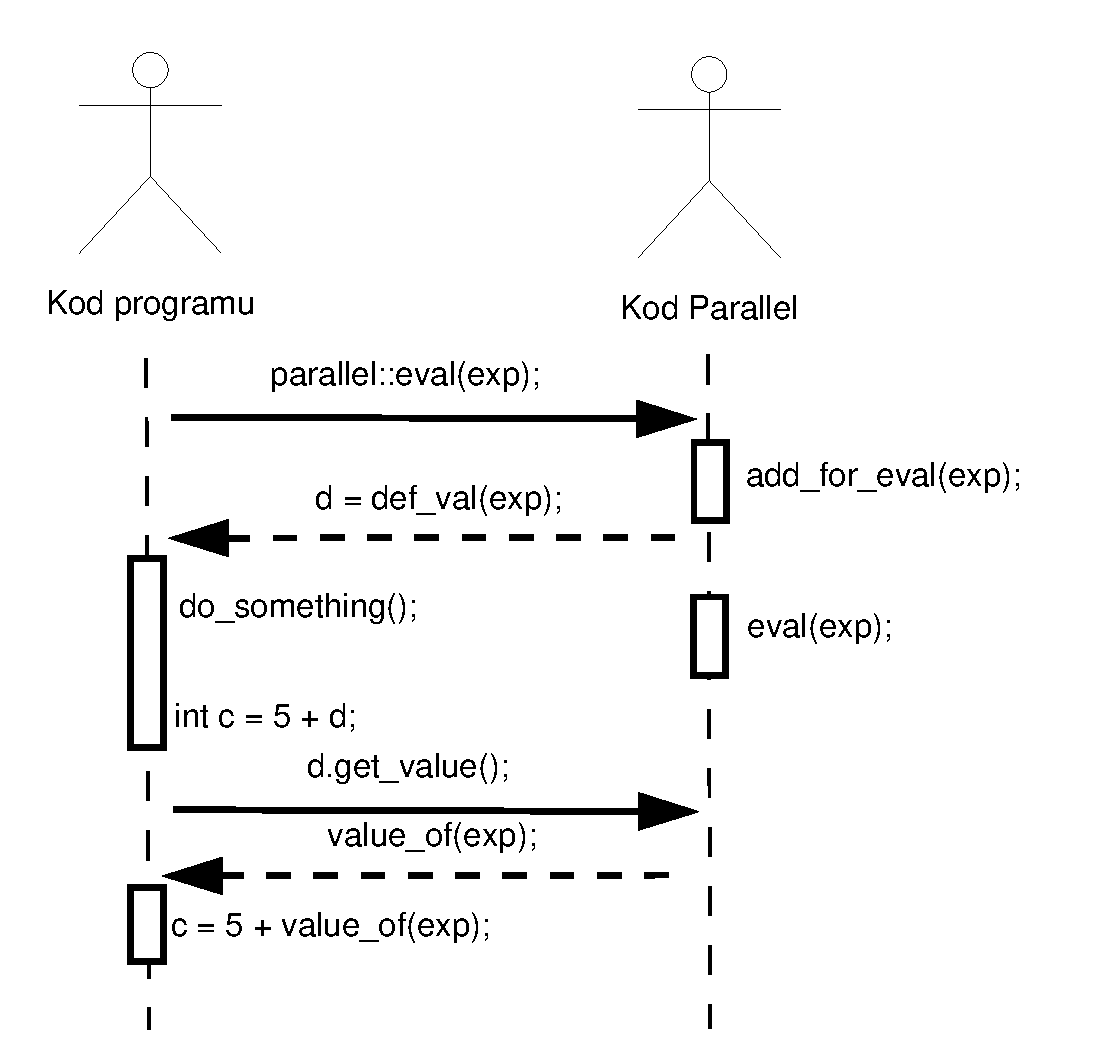
\includegraphics[width=\textwidth]{interaction.eps}
 \caption{Schemat interakcji z bibliotek� Parallel}
\end{figure}

  Schemat pokazuje jak w pierwszej kolejno�ci kod programu wywo�uje funkcj� \feval, kt�ra s�u�y do zlecenia obliczenia r�wnoleg�ego wyra�enia.
  Nast�pnie sterowanie przechodzi do cia�a funkcji \feval, czyli do kodu biblioteki Parallel.
  Funkcja \feval tworzy niezb�dne struktury danych oraz dodaje wyra�enie \verb|exp| do wyra�e� czekaj�cych na wyliczenie.
  Potem nast�puje powr�t z funkcji \feval ze zwr�ceniem warto�ci odroczonej \verb|d| i na jaki� czas kod programu i biblioteki Parallel zaprzestaj� komunikacji.
  Program wykonuje w�asne instrukcje, a biblioteka Parallel wykonuje w�asne, mi�dzy innymi wyliczaj�c wyra�enia, kt�re zosta�y przekazane do wyliczenia r�wnoleg�ego.
  Takie wyliczenie zachodzi w pewnym momencie r�wniez dla wyra�enia \verb|exp|.
  
  Gdy potrzebna jest wyliczona warto�� wyra�enia \verb|exp| nast�puje automatycznie pr�ba pobrania warto�ci wyra�enia z warto�ci odroczonej \verb|d|.
  Wtedy sterowanie przechodzi do kodu biblioteki, kt�ry przekazuje z powrotem wyliczon� warto�� wyra�enia \verb|exp|.
  Kod programu otrzymuje warto�� i mo�e dalej prowadzi� swoje obliczenia.
  Tak wygl�da jeden cykl skorzystania z mechanizmu zlecania wyra�e� do r�wnoleg�ego wyliczenia w bibliotece Parallel.
  
\clearpage
 
\section{Istniej�ce biblioteki do programowania r�wnoleg�ego w j�zyku C++}

  W tej sekcji opis idei biblioteki Parallel zestanie przeciwstawiony przegl�dowi obecnie istniej�cych bibliotek do programowania wsp�bie�nego w jezyku C++.
  Powsta�o ich wiele, o r�nych cechach, jednak �adna z nich nie realizuje zestawu cel�w, kt�ry postawi�em przed bibliotek� Parallel.
  Dlatego, moim zdaniem, istnia�a potrzeba stworzenia nowej biblioteki, kt�ra r�ni si� znacznie od istniej�cych rozwiaza� i pokrywa inny zakres potrzeb programist�w.
  Sw�j przegl�d opr� na przegl�dzie najpopularniejszych bibliotek do programowania r�wnoleg�ego w C++ dokonany na podstawie ich dokumentacji oraz publikacji naukowych.
  
\subsection{Open Multi-Processing (OpenMP)}

  OpenMP zosta� stworzony do pisania wielow�tkowych program�w w  dla system�w wieloprocesorowych z pami�ci� dzielon�.
  Dzi�ki temu, �e zosta� uzgodniony przez najwi�ksze firmy dostarczaj�ce oprogramowanie i sprz�t komputerowy wspiera wiele platform, takich jak Microsoft Windows, Unix, oraz wiele j�zyk�w, na przyk�ad C, C++, Fortran.
  
  Nie jest typow� bibliotek�, gdy� opr�cz pewnego zbioru funkcji udost�pnia r�wnie� zbi�r dyrektyw kompilatora raz zmiennych �rodowiskowych, kt�re modyfikuj� dzia�anie programu.
  Programowanie odbywa si� w spos�b jawny, to znaczy programista wyra�nie opisuje w kodzie jak powinno przebiega� r�wnoleg�e wykonanie programu.
  Ten opis dokonywany jest w wi�kszo�ci przez u�ycie odpowiednich dyrektyw kompilatora.
  Oczywi�cie nie wszystkie kompilatory zgodne ze standardem C++, wspieraj� OpenMP, to wsparcie musia�o zosta� specjalnie do��czone, tak aby kompilator rozumia� dyrektywy i kierowany tymi dyrektywami m�g� wygenerowa� wsp�bie�ny kod.
  
  Oto prosty przyk�ad kodu napisanego przy pomocy OpenMP:
  \begin{lstlisting}
#include <omp.h>
#include <iostream>
int main (int argc, char *argv[]) {
 int th_id, nthreads;
#pragma omp parallel private(th_id)
 {
  th_id = omp_get_thread_num();
  std::cout << "Hello World from thread" << th_id << "\n";
#pragma omp barrier
 if ( th_id == 0 ) {
   nthreads = omp_get_num_threads();
   std::cout << "There are " << nthreads << " threads\n";
  }
 }
 return 0;
}
  \end{lstlisting}
  Program wypisuje komunikat ``Hello World'' z do��czonym numerem w�tku. 
  Zr�wnoleglenie tego kodu przez kompilator osi�gni�to stosuj�c dyrektyw� \verb|#pragma omp parallel private(th_id)|.
  Wynika z niej, �e kompilator powinien zr�wnolegli� zaznaczony blok kodu, przy czym zmienna \verb|th_id| ma by� prywatna, czyli ka�dy w�tek powinien posiada� swoj� kopi�.

  OpenMP wykorzystuje model Fork-Join.
  W programie napisanym przy u�yciu OpenMP wyst�puje w�tek g�owny, kt�ry koordynuje prac�.
  Gdy wykonanie dochodzi do pocz�tku regionu kodu, kt�ry zosta� oznaczony odpowiednimi dyrektywami do zr�wnoleglenia, wtedy nast�puje faza fork, czyli tworzenia w�tk�w.
  Ka�dy z w�tk�w otrzymuje unikalny identyfikator, kt�rego warto�� mo�na odczyta� i przy jego pomocy sterowa� prac� tylko okre�lonego w�tku.
  W�tki przetwarzaj� kod przeznaczony do zr�wnoleglenia niezale�nie od siebie, aczkolwiek istniej� mechanizmy pozwalaj�ce na zdefiniowany przez programist� podzia� zada�.
  Dzi�ki temu mo�liwe jest zr�wnoleglenie zar�wno na poziomie zada�, r�ne w�tki mog� wykonywa� r�ny kod, jak i na poziomie danych, gdy w�tki wykonuj� ten sam kod, ale na r�nych danych.
  Nast�pnie w�tki wykonuj� zadanie, po czym na ko�cu kodu zaznaczonego do zr�wnoleglenia nast�puje faza-join, w kt�rej w�tek g��wny oczekuje na zako�czenie pracy wszystkich w�tk�w pracownik�w.
  Liczba w�tk�w mo�e by� kontrolowana przez programist� za pomoc� funkcji OpenMP lub zmiennych �rodowiskowych.
  
  Kolejny prosty przyk�ad pokazuje jak w OpenMP mo�na wykona� dodawanie dw�ch tablic:
\begin{lstlisting}
#include <omp.h>
#define CHUNKSIZE 100
#define N     1000

main ()  
{

int i, chunk;
float a[N], b[N], c[N];

/* Some initializations */
for (i=0; i < N; i++)
  a[i] = b[i] = i * 1.0;
chunk = CHUNKSIZE;

#pragma omp parallel shared(a,b,c,chunk) private(i)
  {

  #pragma omp for schedule(dynamic,chunk) nowait
  for (i=0; i < N; i++)
    c[i] = a[i] + b[i];

  }  /* end of parallel section */

}
\end{lstlisting}
  W tym przyk�adzie nast�puje zr�wnowleglenie p�tli for, w kt�rej sumowane s� elementy dw�ch tablic i wynik przypisywany jest na trzeci� tablic�.
  Dyrektywa \verb|#pragma omp for schedule(dynamic,chunk) nowait| m�wi, i� p�tla powinna zosta� zr�wnoleglona, 
  ale w taki spos�b, �e ka�dy z w�tk�w zajmie si� fragmentem tablicy o wielko�ci zapisanej w zmiennej \verb|chunk|.
  Kolejne obroty p�tli nie s� ze sob� synchronizowane, o czym m�wi s�owo \verb|nowait|.
  
\subsubsection{Por�wnanie OpenMP vs. Parallel}

\begin{tabular}{ | p{0.5\textwidth} | p{0.5\textwidth} |}
  \hline\
  \textbf{Podobie�stwa} & \textbf{R�nice} \\ \hline
  \begin{itemize}
   \item R�wnoleg�o�� inkrementacyjna, mo�liwe jest dodawanie zr�wnoleglania oblicze� stopniowo, bez drastycznych zmian w kodzie.
   \item Ma�a potrzeba zmian w kodzie przy zr�wnoleglaniu
   \item W obu przypadkach mo�liwa jest kompilacja do kodu sekwencyjnego bez �adnych modyfikacji w kodzie.
   \item OpenMP i Parallel dzia�aj� tylko na platformach z pami�ci� wsp�dzielon�.
  \end{itemize}

  &
  \begin{itemize}
   \item W OpenMP dekompozycja zada� domy�lnie jest dokonywana automatycznie
   \item OpenMP nie jest zwyk�� bibliotek� j�zyka i potrzebuje wsparcia kompilatora.
   \item Parallel zosta�o zaprojektowane do zr�wnoleglania zadaniowego, a nie zr�wnoleglania na poziomie danych (ni�sza ziarnisto��). W OpenMP oba te podej�cia s� wspierane.
   \item OpenMP nie wspiera obs�ugi wyj�tk�w, a biblioteka Parallel tak.
   \item OpenMP pozwala na mniejsz� dowolno�� synchronizacji r�wnoleg�ych fragment�w kodu. W Parallel w�tki s� synchronizowane, gdy jest to niezb�dne.
  \end{itemize}\\
  \hline
\end{tabular} 

\subsection{Threading Building Blocks (TBB)}

  Threading Building Blocks jest bibliotek�, kt�ra s�u�y do pisania program�w wykorzystuj�cych wielow�tkowo�� w j�zyku C++.
  Biblioteka sk�ada si� z szablon�w typ�w i algorytm�w, kt�re dzia�aj� w spos�b r�wnoleg�y, jednocze�nie pozwalaj� unikn�� trudno�ci i z�o�ono�ci zwi�zanych z programowaniem 
  przy wykorzystaniu standardowych mechanizm�w oferuj�cych r�wnoleg�o��, takich jak w�tki POSIX, Windows lub w�tki z biblioteki Boost.Thread.
  W standardowej bibliotece oferuj�cej wielow�tkowo�� programista obcia�ony jest tworzeniem, usuwaniem lub synchronizacj� w�tk�w i przypisywaniem do nich zada�.
  
  W przypadku TBB programista, zamiast definowa� dzia�anie wsp�bie�nego fragmentu programu manualnie, u�ywa szkielet�w algorytm�w dost�pnych w tej biblioitece.
  Nast�pnie biblioteka ju� sama dzieli wykonanie algorytmu na podzadania, przypisuje je do w�tk�w, 
  zajmuje si� r�wnowa�eniem obci��enia procesor�w i przypisywaniem w�tk�w do procesor�w w taki spos�b, by zminimalizowa� migotanie pami�ci podr�cznej.
  Nawet liczba w�tk�w jest dobierana automatycznie przez TBB zale�nie od konfiguracji komputera.
  
  Przyk�ad wykorzystania biblioteki TBB do zr�wnoleglenia p�tli for wygl�da nast�puj�co:
  \begin{lstlisting}
#include "tbb/blocked_range.h"

class ApplyFoo {
  float *const my_a;
  public:
    void operator()( const blocked_range<size_t>& r ) const {
      for( size_t i=r.begin(); i!=r.end(); ++i ) {
        Foo(my_a[i]);     
      }
    }
  ApplyFoo( float a[] ) :
    my_a(a) {}
};

#define A_SIZE 1000
int main() 
{
  float a[A_SIZE];
  parallel_for(blocked_range<size_t>(0,n,IdealGrainSize), 
    ApplyFoo(a) );
}
  \end{lstlisting}
  W tym przyk�adzie klasa ApplyFoo definiuje obiekt funkcyjny, kt�ry je�li otrzyma za argument obiekt typu \verb|blocked_range<size_t>| 
  to przypisze na ka�dy element tablicy \verb|my_a| warto�� zwracan� przez wywo�anie funkcji \verb|Foo| od tego elementu.
  Poni�ej w funkcji \verb|main| znajduje si� wywo�anie funkcji TBB \verb|parallel_for|, kt�ra r�wnolegle aplikuje obiekt funkcyjny \verb|ApplyFoo(a)|
  do fragment�w tablicy \verb|a| wielko�ci \verb|IdealGrainSize|.
  
  TBB zawiera, opr�cz schematu p�tli for, r�wnie� wiele innych: schemat p�tli while, schemat pipeline, schemat reduce.
  
\subsubsection{Por�wnanie TBB vs. Parallel}

\begin{tabular}{ | p{0.5\textwidth} | p{0.5\textwidth} |}
  \hline\
  \textbf{Podobie�stwa} & \textbf{R�nice} \\ \hline
  \begin{itemize}
   \item R�wnoleg�o�� inkrementacyjna, mo�liwe jest dodawanie zr�wnoleglania oblicze� stopniowo, bez drastycznych zmian w kodzie.
   \item TBB i Parallel dzia�aj� tylko na platformach z pami�ci� wsp�dzielon� i nie jest mo�liwe przeskalowanie programu na wiele maszyn.
   \item Obie biblioteki zosta�y zaprojektowane do zr�wnoleglania kodu na poziomie zada� do wykonania.
   \item Obie biblioteki wspieraj� obs�ug� wyj�tk�w.
  \end{itemize}

  &
  \begin{itemize}
   \item U�ycie TBB zazwyczaj wymaga zmian w kodzie. Cho� jego struktura pozostaje w wi�kszo�ci niezmieniona, to niezb�dne jest zdefinowanie klas - obiekt�w funkcyjnych przekazywanych do algorytm�w z TBB.
   \item Kod TBB jest mniej czytelny, gdy� to co si� dzieje w programie opisane jest w miejscu wywo�uj�cym r�wnoleg�e wykonanie, jak i przez obiekty funkcyjne przekazywane do TBB zdefinowane w innym miejscu w kodzie.
   \item W TBB dekompozycja zada� domy�lnie jest dokonywana automatycznie.
   \item Kod pisany przy u�yciu TBB zazwyczaj jest d�u�szy, ze wzgl�du na konieczno�� definowania dodatkowych klas.
  \end{itemize}\\
  \hline
\end{tabular} 

\subsection{Message Passing Interface (MPI)}

  Message Passing Interface jest bibliotek� nieco odmienn� od poprzednio opisanych, gdy� pozwala na pisanie program�w r�wnoleg�ych na systemy komputerowe z pami�ci� rozproszon�.
  Jest to mo�liwe dzi�ki komunikacji poprzez wiadomo�ci, kt�r� zapewnia biblioteka.
  W typowym przypadku program r�wnoleg�y sk�ada si� z wielu proces�w komunikuj�cych si� poprzez wywo�ania odpowiednich funkcji MPI do wysy�ania lub odbierania wiadomo�ci.
  MPI zosta�o ustandaryzowane i jest dost�pne w wielu j�zykach i na wielu platformach.
  
  MPI uwa�ane jest za dosy� niskopoziomowy spos�b pisania program�w r�wnoleg�ych, gdy� ca�e dzia�anie programu musi zosta� zapisane jawnie przez programist�.
  Programista ustala liczb� proces�w, kierunki komunikacji, mechanizmy synchronizacji, podzia� danych i ich rozk�ad pomi�dzy procesy oraz
  przydzia� proces�w do procesor�w.
  Jako korzy�� z trudno�ci programowania przy pomocy MPI mo�na zaliczy� wydajno�� z jak� dzia�aj� dobrze napisane programy oraz �atwo�� z jak� mo�na skalowa� je na wi�ksz� liczb� procesor�w.
  Ponadto dzi�ki szerokiemu wsparciu MPI przez najwi�kszych dostawc�w sprz�tu i oprogramowania, programy pisane przy pomocy MPI s� przeno�ne.
  
  Oto przyk�ad programu napisanego przy pomocy MPI, kt�ry pokazuje podstawowe operacje zwi�zane z wysy�aniem i odbieraniem komunikat�w.
\begin{lstlisting}
/*
 * "Hello World" MPI Test Program
 */
#include <mpi.h>
#include <stdio.h>
#include <string.h>

#define BUFSIZE 128
#define TAG 0

int main(int argc, char *argv[])
{
 char idstr[32];
 char buff[BUFSIZE];
 int numprocs;
 int myid;
 int i;
 MPI_Status stat;
 
 /* kazdy program MPI musi najpierw wywolac MPI_Init */
 MPI_Init(&argc,&argv); 
 /* sprawdzenie ile jest procesow w grupie */
 MPI_Comm_size(MPI_COMM_WORLD,&numprocs); 
 /* sprawdzenie numeru danego procesu w grupie */
 MPI_Comm_rank(MPI_COMM_WORLD,&myid); 
 
 if(myid == 0)
 {
   printf("%d: We have %d processors\n", myid, numprocs);
   for(i=1;i<numprocs;i++)
   {
     sprintf(buff, "Hello %d! ", i);
     MPI_Send(buff, BUFSIZE, MPI_CHAR, i, TAG, MPI_COMM_WORLD);
   }
   for(i=1;i<numprocs;i++)
   {
     MPI_Recv(buff, BUFSIZE, MPI_CHAR, i, TAG, 
      MPI_COMM_WORLD, &stat);
     printf("%d: %s\n", myid, buff);
   }
 }
 else
 {
   /* odebranie wiadomosci od procesu o identyfikatorze 0 */
   MPI_Recv(buff, BUFSIZE, MPI_CHAR, 0, TAG, 
    MPI_COMM_WORLD, &stat);
   sprintf(idstr, "Processor %d ", myid);
   strncat(buff, idstr, BUFSIZE-1);
   strncat(buff, "reporting for duty\n", BUFSIZE-1);
   /* wys�anie wiadomo�ci do procesu z identyfikatorem 0 */
   MPI_Send(buff, BUFSIZE, MPI_CHAR, 0, TAG, MPI_COMM_WORLD);
 }

 /* Program MPI powinien zakonczy� si� wywo�aniem MPI_Finalize, 
  * ktory jest dla procesow punktem synchronizacji. 
  */
 MPI_Finalize(); 
 return 0;
}
\end{lstlisting}
  W tym programie w�tek g��wny o identyfikatorze 0 wysy�a wiadomo�� ``Hello'' do ka�dego z w�tk�w, a nast�pnie oczekuje na odpowied� od wszystkich w�tk�w.
  W�tki pozosta�e czekaj� na wiadomo��, a nast�pnie wysy�aj� odpowied�.
  
  Kod pokazuje, �e programowanie w MPI mo�na uzna� za dosy� niskopoziomowe. 
  Operacje wysy�ania i odbierania wiadomo�ci dzia�aj� analogicznie do funkcji systemowych read i write, operuj� na poziomie bit�w.
  St�d programista powinien tak�e zatroszczy� si� o odpowiednie zakodowanie i rozkodowanie wiadomo�ci.
  
\subsubsection{Por�wnanie MPI vs. Parallel}

\begin{tabular}{ | p{0.5\textwidth} | p{0.5\textwidth} |}
  \hline\
  \textbf{Podobie�stwa} & \textbf{R�nice} \\ \hline
  \begin{itemize}
   \item Obie biblioteki zosta�y zaprojektowane do zr�wnoleglania kodu na poziomie zada� do wykonania.
  \end{itemize}

  &
  \begin{itemize}
   \item W MPI raczej trudno jest stopniowo zr�wnolegla� program. Fragmeny programu, kt�re maj� dzia�a� r�wnoleg�e musz� zosta� zapisane w ca�o�ci i musz� dok�adnie sobie odpowiada�.
   \item MPI wymaga znacznych strukturalnych zmian w kodzie.
   \item Ze wzgl�du na to, �e MPI koordynuje prac� wielu niezale�nych proces�w, kt�re dzia�aj� w spos�b asynchroniczny trudno jest dok�adnie prze�ledzi� i zrozumie� dzia�anie takiego programu.
   \item MPI dzia�a tak�e w systemach komputerowych z pami�ci� rozproszon�, Parallel tylko w �rodowisku z pami�ci� dzielon�.
   \item W MPI ca�o�� komunikacji, synchronizacji, podzia� zada�, zbieranie wynik�w musi zosta� zapisane \textit{explicite} przez programist�.
   \item Komunikacja w MPI odbywa si� pomi�dzy r�nymi procesami, a w Parallel pomi�dzy w�tkami o wsp�lnej przestrzeni adresowej. MPI mo�na stosowa� w og�lniejszych przypadkach.
  \end{itemize}\\
  \hline
\end{tabular} 

\subsection{Boost Threads}

  Istnieje kilka bibliotek oferuj�cych programi�cie mo�liwo�� uruchamiania wielu watk�w w ramach jednego programu.
  W�r�d nich mo�na wymieni� POSIX Threads, Windows Threads, najbardziej typowe rozwi�zania dla platform odpowiednio Unix i Windows.
  Do opisu zosta�a Boost.Threads ze wzgl�du na przenaszalno��, natomiast zasada dzia�ania i oferowane mo�liwo�ci s� analogicznie jak w innych tego typu bibliotekach.
  
  Biblioteka Boost Threads umo�liwia zarz�dzanie w�tkami, jak i udost�pnia typy oraz funkcje s�u��ce do synchronizacji pomi�dzy w�tkami.
  Mechanizmy synchronizacyjne dost�pne w Boost Thread to mi�dzy innymi r�nego rodzaju blokady, zmienne warunkowe, bariery.
  Boost Thread pozwala r�wnie� na tworzenie grup w�tk�w, kt�rymi mo�na zarz�dza�, ale nie ma funkcji puli w�tk�w, kt�ra optymalizowa�aby zu�ycie zasob�w przy pos�ugiwaniu si� w�tkami.
  Komunikacja w programie pisanym przy u�yciu Boost Thread odbywa si� zazwyczaj przez wsp�dzielone struktury danych, o ochron� kt�rych programista musi zatroszczy� si� samodzielnie.
  
  Poni�ej znajduje si� przyk�ad prezentuj�cy u�ycie biblioteki Boost Threads:
\begin{lstlisting}
 
\end{lstlisting}


\subsubsection{Por�wnanie Boost Threads vs. Parallel}

\begin{tabular}{ | p{0.5\textwidth} | p{0.5\textwidth} |}
  \hline\
  \textbf{Podobie�stwa} & \textbf{R�nice} \\ \hline
  \begin{itemize}
   \item Boost Threads i Parallel dzia�aj� tylko na platformach z pami�ci� wsp�dzielon� i nie jest mo�liwe przeskalowanie programu na wiele maszyn.
   \item Obie biblioteki zosta�y zaprojektowane do zr�wnoleglania kodu na poziomie zada� do wykonania.
   \item W przypadku u�ycia obu bibliotek programista musi zadba� o dekompozycje zada�.
  \end{itemize}
  &
  \begin{itemize}
   \item Stopniowe dodawanie r�wnoleg�o�ci przy u�yciu Boost Threads jest trudniejsze, poniewa� u�ycie biblioteki wymaga zmian w strukturze kodu i dodania mechanizmu komunikacji mi�dzy w�tkami.
   \item Nie ma mo�liwo�ci przekazania do w�tku wyra�enia do wykonania, w�tki przyjmuj� do wykonania jedynie obiekty funkcyjne, co wi��e si� z konieczno�ci� dodania do kodu definicji tych obiekt�w.
   \item Kod Boost Threads jest mniej czytelny, gdy� sk�adnia obiekt�w funkcyjnych jest mniej czytelna ni� sk�adnia wyra�e�.
   \item Przekazywanie warto�ci mi�dzy w�tkami wymaga dodatkowej synchronizacji i u�ycia specjalnych fragment�w pami�ci wsp�dzielonej lub wska�nik�w.
   \item W Parallel zadania s� przydzielane w�tkom dynamicznie, dzieki czemu r�wnowa�one jest obci��enie w�tk�w.
   \item Programista u�ywaj�cy Parallel jest w znacznym stopniu odci��ony z u�ywania mechanizm�w synchronizacji i komunikacji pomi�dzy w�tkami.
   \item W Boost Thread wyj�tki wywo�ane w kodzie wykonywanym przez w�tek nie s� sygnalizowane w�tkowi g��wnemu, kt�ry uruchomi� dany w�tek. Mo�na taki efektu uzyska� pisz�c dodatkowy do przekazywania wyj�tk�w pomi�dzy w�tkami.
  \end{itemize}\\
  \hline
\end{tabular} 


\newpage
\section{Zaawansowane przyk�ady u�ycia biblioteki Parallel}

  Opis koncepcji biblioteki Parallel zako�cz� pokazaniem zaawansowanych przyk�ad�w wykorzystania biblioteki Parallel do prowadzenia r�wnoleg�ych oblicze�.
  W pierwszym z przyk�ad�w zaprezentuj�, w jaki spos�b biblioteka Parellel mo�e s�u�y� do zr�wnoleglenia algorytmu szybkiego sortowania (z ang. quicksort).
  Drugi przyk�ad, wykorzystuj�cy w jeszcze wi�kszej mierze mo�liwo�ci biblioteki Parallel, poka�e zdecydowan� przewag� biblioteki Parallel nad standardow� bibliotek� do obs�ugi w�tk�w Boost Thread.
  
\subsection{R�wnoleg�e szybkie sortowanie}

  Moja implementacja zr�wnoleglonego szybkiego sortowania opiera si� na prostej idei ``dziel i zwyci�aj''. 
  W ka�dym rekurencyjnym wywo�aniu funkcji sortuj�cej na pocz�tku wywo�ywana jest funkcja \verb|partition|, 
  dziel�ca tablic� na cz�ci o elementach mniejszych od pewnego wyr�nionego elementu i o elementach wi�kszych od tego� elementu.
  Nast�pnie, je�li podtablice do posortowania s� wystarczaj�co du�e (w przyk�adzie limit zosta� ustalony na 100 element�w), wywo�ywana jest rekurencyjnie funkcja sortuj�ca.
  W przeciwnym przypadku, tablica jest sortowana standardowym algorytmem sekwencyjnym szybkiego sortowania.
  
  W celu por�wnania biblioteki Parallel z ju� istniej�cym rozwi�zaniem, implementacje dostarczy�em w dw�ch wersjach
  Jedna jest zaimplementowana przy u�yciu biblioteki Boost Thread, a druga przy u�yciu biblioteki Parallel.
  Oto implementacja wykorzystuj�ca standardow� bibliotek� do obs�ugi wielow�tkowo�ci Boost Thread:
  \begin{lstlisting}
const unsigned limit = 100;
  
template <typename Item>
void thread_quicksort(Item array[], size_t l, size_t r)
{
  if (l < r)
  {
    size_t s = partition(array, l, r);
    boost::thread thread;
    if (s - l > limit) 
      thread = boost::thread(
	boost::bind(quicksort<int>, array, l, s - 1));
    else
      quicksort(array, l, s - 1);
    quicksort(array, s + 1, r);
    if (s - l > limit)
      thread.join();
  }
}
  \end{lstlisting}
  
  Jak mo�na zauwa�y�, dla ka�dego r�wnoleg�ego wywo�ania funkcji \verb|thread_quicksort| musi zosta� stworzony w�tek, poniewa� Boost Thread nie posiada puli w�tk�w.
  \footnote{Oczywi�cie pul� w�tk�w mo�na zaimplementowa� wykorzystuj�c Boost Thread, ale moim celem by�o pokazanie przyk�ad�w zr�wnoleglenia szybkiego sortowania, 
  kt�rych napisanie by�o podobne pod wzgl�dem struktury kodu i pracoch�onno�ci.}
  W przypadu du�ych tablic mo�e to skutkowa� spowolnieniem dzia�ania programu z powodu zbyt du�ego obci��enia systemu w�tkami i zbyt cz�stych prze��cze� kontekstu.
  
  Poni�szy kod pokazuje implementacj� szybkiego sortowania, korzystaj�c� z biblioteki Parallel:
  \begin{lstlisting}
const unsigned limit = 100;
  
template <typename Item>
void parallel_quicksort(Item array[], size_t l, size_t r)
{
  if (l < r)
  {
    size_t s = partition(array, l, r);
    deferred_value<void> tmp;
    if (s - l > limit)
      tmp = parallel::eval(
	parallel::lazyf(quicksort<int>, array, l, s - 1));
    quicksort(array, s + 1, r);
    if (s - l > limit)
      tmp.force();
  }
}
  \end{lstlisting}
  
  Implementacja bazuj�ca na Parallel ma przewag� polegaj�c� na tym, �e w�tki s� tworzone tylko raz podczas inicjalizacji biblioteki Parallel.
  Zatem nie jest mo�liwe przeci��enie systemu niekontrolowanym rozmno�eniem si� w�tk�w.
  Poza istotn� korzy�ci� zwi�zan� z brakiem potrzeby zarz�dzania w�tkami, w samej strukturze programu nie wida� znacz�cych korzy�ci z wyboru biblioteki Parallel.
  Kod wygl�da bardzo podobnie.
  Aby uwypukli� zalety Parallel w por�wnaniu ze standardowymi bibliotekami b�dzie potrzebny kolejny przyk�ad.

\subsection{R�wnoleg�e sumowanie element�w tablicy}

  Przyk�ad zr�wnoleglenia sumowania element�w tablicy poka�e jak wygodna jest sk�adnia bibioteki Parallel 
  w por�wnianiu ze sk�adni� biblioteki Boost.Threads, gdy r�wnoleg�e obliczenia zwracaj� pewn� warto��.
  
  Implementacja wielow�tkowa, napisana w oparciu o Boost.Threads, wygl�da nast�puj�co:
  \begin{lstlisting}
void sum(int* wynik, int* begin, int* end)
{
  *wynik = 0;
  for (int* i = begin; i != end; i++) *wynik += *i;
}  

int array_sum_thread(int* array, size_t size)
{
  int s1, s2, s3, s4;
  boost::thread t1(
    boost::bind(sum, &s1, array, array + size/4));
  boost::thread t2(
    boost::bind(sum, &s2, array + size/4 + 1, array + size/2));
  boost::thread t3(
    boost::bind(sum, &s3, array + size/2 + 1, 3*size/4));
  boost::thread t4(
    boost::bind(sum, &s4, array + 3*size/4 + 1, array + size));
  t1.join();
  t2.join();
  t3.join();
  t4.join();
  return s1 + s2 + s3 + s4;
}
  \end{lstlisting}
  W tej implementacji niezb�dne by�o zdefiniowanie funkcji sumuj�cej pewien odcinek tablicy, kt�ra zwraca wynik przez jeden z argument�w,
  poniewa� w�tki nie potrafi� zwr�ci� �adnych warto�ci.
  Oczywi�cie, w przypadku tak prostej implementacji nie ma mo�liwo�ci obs�ugi b��d�w, kt�re mog� pojawi� si� podczas oblicze�.
  Ponadto programista musia� zadba� o synchronizacj� w�tk�w, w tym przypadku poprzez wywo�anie funkcji \verb|join| na ka�dym z w�tk�w,
  aby zagwarantowa�, �e ka�dy z nich zako�czy� si� przed zsumowaniem rezultat�w podzada�.
  
  Poni�ej znajduje si� kod wykonuj�cy to samo zadanie, ale napisany przy pomocy biblioteki Parallel:
  \begin{lstlisting}
int sum(int* begin, int* end)
{
  int s = 0;
  for (int* i = begin; i != end; i++) s += *i;
  return s;
}
  
int array_sum_parallel(int* array, size_t size)
{
  deferred_value<in> sum = parallel::evaluate(
    *parallel::lazyf(sum, array, array + size/4));
  for (int i = 1; i < 4; i++)
  {
    sum += parallel::evaluate(parallel::lazyf(
      sum, array + (i * size)/4 + 1, array + ((i+1) * size)/4));
  }
  return sum;
}
  \end{lstlisting}
  W tym przyk�adzie, funkcja sumuj�ca tablic� ma bardziej naturaln� posta�, w kt�rej wynik zwracany jest w standardowy spos�b.
  W zwi�zku z tym, cz�sto w praktycznych zastosowaniach b�dzie mo�na u�y� ju� istniej�cej funkcji, co zmniejszy pracoch�onno�� pisania program�w i u�atwi unikni�cie b��d�w.
  W kodzie programu nie wida� �adnego �ladu jawnej synchronizacji pomi�dzy w�tkami, gdy� dzi�ki odpowiedniej implementacji warto�ci odroczonych synchronizacja zarz�dzana jest automatycznie przez bibliotek�.
  Pomimo tego, �e w linii 13. przyk�adu warto�� sum jest u�ywana, to prze�adowanie operatora \verb|+=| sprawia, �e obliczenie warto�ci odroczonej nie jest wymuszane
  i wszystkie podzadania wykonuj� si� r�wnocze�nie.
  Dopiero w linii 15, gdzie warto�� odroczona \verb|sum| jest konwertowana do \verb|int| nast�puje pobranie wyniku ze wszystkich zleconych oblicze� i zwr�cenie warto�ci.
  Warto r�wnie� zauwa�y�, �e kod napisany przy pomocy biblioteki Parallel jest bardziej czytelny i kr�tszy.
 

%   Programista w celu wykorzystania możliwości równoległego musi dokonać wyboru modelu programowania równoległego, narzędzi, które ten model wspierają, 
%   a następnie do dokonanych decyzji zaprojektować program.
%   Proces projektowania programu równoległego jest znacznie bardziej skomplikowany niż programu sekwencyjnego, ze względu na to, 
%   że zazwyczaj narzędzia do programowania równoległego narzucają strukturę programu, która w znacznym stopniu różni się od programu sekwencyjengo, 
%   nie jest tak naturalna, a przez to trudniejsza do wykonania i zrozumienia.
%   Dwa podstawowe problemy, które towarzyszą wyborowi technologii do programowania równoległego, to poziom abstrakcji oraz wydajność.
%   Poziom abstrakcji

\section{Istniej�ce biblioteki do programowania r�wnoleg�ego w j�zyku C++}

  W tej sekcji opis idei biblioteki Parallel zestanie przeciwstawiony przegl�dowi obecnie istniej�cych bibliotek do programowania wsp�bie�nego w jezyku C++.
  Powsta�o ich wiele, o r�nych cechach, jednak �adna z nich nie realizuje zestawu cel�w, kt�ry postawi�em przed bibliotek� Parallel.
  Dlatego, moim zdaniem, istnia�a potrzeba stworzenia nowej biblioteki, kt�ra r�ni si� znacznie od istniej�cych rozwiaza� i pokrywa inny zakres potrzeb programist�w.
  Sw�j przegl�d opr� na przegl�dzie najpopularniejszych bibliotek do programowania r�wnoleg�ego w C++ dokonany na podstawie ich dokumentacji oraz publikacji naukowych.
  
\subsection{Open Multi-Processing (OpenMP)}

  OpenMP zosta� stworzony do pisania wielow�tkowych program�w w  dla system�w wieloprocesorowych z pami�ci� dzielon�.
  Dzi�ki temu, �e zosta� uzgodniony przez najwi�ksze firmy dostarczaj�ce oprogramowanie i sprz�t komputerowy wspiera wiele platform, takich jak Microsoft Windows, Unix, oraz wiele j�zyk�w, na przyk�ad C, C++, Fortran.
  
  Nie jest typow� bibliotek�, gdy� opr�cz pewnego zbioru funkcji udost�pnia r�wnie� zbi�r dyrektyw kompilatora raz zmiennych �rodowiskowych, kt�re modyfikuj� dzia�anie programu.
  Programowanie odbywa si� w spos�b jawny, to znaczy programista wyra�nie opisuje w kodzie jak powinno przebiega� r�wnoleg�e wykonanie programu.
  Ten opis dokonywany jest w wi�kszo�ci przez u�ycie odpowiednich dyrektyw kompilatora.
  Oczywi�cie nie wszystkie kompilatory zgodne ze standardem C++, wspieraj� OpenMP, to wsparcie musia�o zosta� specjalnie do��czone, tak aby kompilator rozumia� dyrektywy i kierowany tymi dyrektywami m�g� wygenerowa� wsp�bie�ny kod.
  
  Oto prosty przyk�ad kodu napisanego przy pomocy OpenMP:
  \begin{lstlisting}
#include <omp.h>
#include <iostream>
int main (int argc, char *argv[]) {
 int th_id, nthreads;
#pragma omp parallel private(th_id)
 {
  th_id = omp_get_thread_num();
  std::cout << "Hello World from thread" << th_id << "\n";
#pragma omp barrier
 if ( th_id == 0 ) {
   nthreads = omp_get_num_threads();
   std::cout << "There are " << nthreads << " threads\n";
  }
 }
 return 0;
}
  \end{lstlisting}
  Program wypisuje komunikat ``Hello World'' z do��czonym numerem w�tku. 
  Zr�wnoleglenie tego kodu przez kompilator osi�gni�to stosuj�c dyrektyw� \verb|#pragma omp parallel private(th_id)|.
  Wynika z niej, �e kompilator powinien zr�wnolegli� zaznaczony blok kodu, przy czym zmienna \verb|th_id| ma by� prywatna, czyli ka�dy w�tek powinien posiada� swoj� kopi�.

  OpenMP wykorzystuje model Fork-Join.
  W programie napisanym przy u�yciu OpenMP wyst�puje w�tek g�owny, kt�ry koordynuje prac�.
  Gdy wykonanie dochodzi do pocz�tku regionu kodu, kt�ry zosta� oznaczony odpowiednimi dyrektywami do zr�wnoleglenia, wtedy nast�puje faza fork, czyli tworzenia w�tk�w.
  Ka�dy z w�tk�w otrzymuje unikalny identyfikator, kt�rego warto�� mo�na odczyta� i przy jego pomocy sterowa� prac� tylko okre�lonego w�tku.
  W�tki przetwarzaj� kod przeznaczony do zr�wnoleglenia niezale�nie od siebie, aczkolwiek istniej� mechanizmy pozwalaj�ce na zdefiniowany przez programist� podzia� zada�.
  Dzi�ki temu mo�liwe jest zr�wnoleglenie zar�wno na poziomie zada�, r�ne w�tki mog� wykonywa� r�ny kod, jak i na poziomie danych, gdy w�tki wykonuj� ten sam kod, ale na r�nych danych.
  Nast�pnie w�tki wykonuj� zadanie, po czym na ko�cu kodu zaznaczonego do zr�wnoleglenia nast�puje faza-join, w kt�rej w�tek g��wny oczekuje na zako�czenie pracy wszystkich w�tk�w pracownik�w.
  Liczba w�tk�w mo�e by� kontrolowana przez programist� za pomoc� funkcji OpenMP lub zmiennych �rodowiskowych.
  
  Kolejny prosty przyk�ad pokazuje jak w OpenMP mo�na wykona� dodawanie dw�ch tablic:
\begin{lstlisting}
#include <omp.h>
#define CHUNKSIZE 100
#define N     1000

main ()  
{

int i, chunk;
float a[N], b[N], c[N];

/* Some initializations */
for (i=0; i < N; i++)
  a[i] = b[i] = i * 1.0;
chunk = CHUNKSIZE;

#pragma omp parallel shared(a,b,c,chunk) private(i)
  {

  #pragma omp for schedule(dynamic,chunk) nowait
  for (i=0; i < N; i++)
    c[i] = a[i] + b[i];

  }  /* end of parallel section */

}
\end{lstlisting}
  W tym przyk�adzie nast�puje zr�wnowleglenie p�tli for, w kt�rej sumowane s� elementy dw�ch tablic i wynik przypisywany jest na trzeci� tablic�.
  Dyrektywa \verb|#pragma omp for schedule(dynamic,chunk) nowait| m�wi, i� p�tla powinna zosta� zr�wnoleglona, 
  ale w taki spos�b, �e ka�dy z w�tk�w zajmie si� fragmentem tablicy o wielko�ci zapisanej w zmiennej \verb|chunk|.
  Kolejne obroty p�tli nie s� ze sob� synchronizowane, o czym m�wi s�owo \verb|nowait|.
  
\subsubsection{Por�wnanie OpenMP vs. Parallel}

\begin{tabular}{ | p{0.5\textwidth} | p{0.5\textwidth} |}
  \hline\
  \textbf{Podobie�stwa} & \textbf{R�nice} \\ \hline
  \begin{itemize}
   \item R�wnoleg�o�� inkrementacyjna, mo�liwe jest dodawanie zr�wnoleglania oblicze� stopniowo, bez drastycznych zmian w kodzie.
   \item Ma�a potrzeba zmian w kodzie przy zr�wnoleglaniu
   \item W obu przypadkach mo�liwa jest kompilacja do kodu sekwencyjnego bez �adnych modyfikacji w kodzie.
   \item OpenMP i Parallel dzia�aj� tylko na platformach z pami�ci� wsp�dzielon�.
  \end{itemize}

  &
  \begin{itemize}
   \item W OpenMP dekompozycja zada� domy�lnie jest dokonywana automatycznie
   \item OpenMP nie jest zwyk�� bibliotek� j�zyka i potrzebuje wsparcia kompilatora.
   \item Parallel zosta�o zaprojektowane do zr�wnoleglania zadaniowego, a nie zr�wnoleglania na poziomie danych (ni�sza ziarnisto��). W OpenMP oba te podej�cia s� wspierane.
   \item OpenMP nie wspiera obs�ugi wyj�tk�w, a biblioteka Parallel tak.
   \item OpenMP pozwala na mniejsz� dowolno�� synchronizacji r�wnoleg�ych fragment�w kodu. W Parallel w�tki s� synchronizowane, gdy jest to niezb�dne.
  \end{itemize}\\
  \hline
\end{tabular} 

\subsection{Threading Building Blocks (TBB)}

  Threading Building Blocks jest bibliotek�, kt�ra s�u�y do pisania program�w wykorzystuj�cych wielow�tkowo�� w j�zyku C++.
  Biblioteka sk�ada si� z szablon�w typ�w i algorytm�w, kt�re dzia�aj� w spos�b r�wnoleg�y, jednocze�nie pozwalaj� unikn�� trudno�ci i z�o�ono�ci zwi�zanych z programowaniem 
  przy wykorzystaniu standardowych mechanizm�w oferuj�cych r�wnoleg�o��, takich jak w�tki POSIX, Windows lub w�tki z biblioteki Boost.Thread.
  W standardowej bibliotece oferuj�cej wielow�tkowo�� programista obcia�ony jest tworzeniem, usuwaniem lub synchronizacj� w�tk�w i przypisywaniem do nich zada�.
  
  W przypadku TBB programista, zamiast definowa� dzia�anie wsp�bie�nego fragmentu programu manualnie, u�ywa szkielet�w algorytm�w dost�pnych w tej biblioitece.
  Nast�pnie biblioteka ju� sama dzieli wykonanie algorytmu na podzadania, przypisuje je do w�tk�w, 
  zajmuje si� r�wnowa�eniem obci��enia procesor�w i przypisywaniem w�tk�w do procesor�w w taki spos�b, by zminimalizowa� migotanie pami�ci podr�cznej.
  Nawet liczba w�tk�w jest dobierana automatycznie przez TBB zale�nie od konfiguracji komputera.
  
  Przyk�ad wykorzystania biblioteki TBB do zr�wnoleglenia p�tli for wygl�da nast�puj�co:
  \begin{lstlisting}
#include "tbb/blocked_range.h"

class ApplyFoo {
  float *const my_a;
  public:
    void operator()( const blocked_range<size_t>& r ) const {
      for( size_t i=r.begin(); i!=r.end(); ++i ) {
        Foo(my_a[i]);     
      }
    }
  ApplyFoo( float a[] ) :
    my_a(a) {}
};

#define A_SIZE 1000
int main() 
{
  float a[A_SIZE];
  parallel_for(blocked_range<size_t>(0,n,IdealGrainSize), 
    ApplyFoo(a) );
}
  \end{lstlisting}
  W tym przyk�adzie klasa ApplyFoo definiuje obiekt funkcyjny, kt�ry je�li otrzyma za argument obiekt typu \verb|blocked_range<size_t>| 
  to przypisze na ka�dy element tablicy \verb|my_a| warto�� zwracan� przez wywo�anie funkcji \verb|Foo| od tego elementu.
  Poni�ej w funkcji \verb|main| znajduje si� wywo�anie funkcji TBB \verb|parallel_for|, kt�ra r�wnolegle aplikuje obiekt funkcyjny \verb|ApplyFoo(a)|
  do fragment�w tablicy \verb|a| wielko�ci \verb|IdealGrainSize|.
  
  TBB zawiera, opr�cz schematu p�tli for, r�wnie� wiele innych: schemat p�tli while, schemat pipeline, schemat reduce.
  
\subsubsection{Por�wnanie TBB vs. Parallel}

\begin{tabular}{ | p{0.5\textwidth} | p{0.5\textwidth} |}
  \hline\
  \textbf{Podobie�stwa} & \textbf{R�nice} \\ \hline
  \begin{itemize}
   \item R�wnoleg�o�� inkrementacyjna, mo�liwe jest dodawanie zr�wnoleglania oblicze� stopniowo, bez drastycznych zmian w kodzie.
   \item TBB i Parallel dzia�aj� tylko na platformach z pami�ci� wsp�dzielon� i nie jest mo�liwe przeskalowanie programu na wiele maszyn.
   \item Obie biblioteki zosta�y zaprojektowane do zr�wnoleglania kodu na poziomie zada� do wykonania.
   \item Obie biblioteki wspieraj� obs�ug� wyj�tk�w.
  \end{itemize}

  &
  \begin{itemize}
   \item U�ycie TBB zazwyczaj wymaga zmian w kodzie. Cho� jego struktura pozostaje w wi�kszo�ci niezmieniona, to niezb�dne jest zdefinowanie klas - obiekt�w funkcyjnych przekazywanych do algorytm�w z TBB.
   \item Kod TBB jest mniej czytelny, gdy� to co si� dzieje w programie opisane jest w miejscu wywo�uj�cym r�wnoleg�e wykonanie, jak i przez obiekty funkcyjne przekazywane do TBB zdefinowane w innym miejscu w kodzie.
   \item W TBB dekompozycja zada� domy�lnie jest dokonywana automatycznie.
   \item Kod pisany przy u�yciu TBB zazwyczaj jest d�u�szy, ze wzgl�du na konieczno�� definowania dodatkowych klas.
  \end{itemize}\\
  \hline
\end{tabular} 

\subsection{Message Passing Interface (MPI)}

  Message Passing Interface jest bibliotek� nieco odmienn� od poprzednio opisanych, gdy� pozwala na pisanie program�w r�wnoleg�ych na systemy komputerowe z pami�ci� rozproszon�.
  Jest to mo�liwe dzi�ki komunikacji poprzez wiadomo�ci, kt�r� zapewnia biblioteka.
  W typowym przypadku program r�wnoleg�y sk�ada si� z wielu proces�w komunikuj�cych si� poprzez wywo�ania odpowiednich funkcji MPI do wysy�ania lub odbierania wiadomo�ci.
  MPI zosta�o ustandaryzowane i jest dost�pne w wielu j�zykach i na wielu platformach.
  
  MPI uwa�ane jest za dosy� niskopoziomowy spos�b pisania program�w r�wnoleg�ych, gdy� ca�e dzia�anie programu musi zosta� zapisane jawnie przez programist�.
  Programista ustala liczb� proces�w, kierunki komunikacji, mechanizmy synchronizacji, podzia� danych i ich rozk�ad pomi�dzy procesy oraz
  przydzia� proces�w do procesor�w.
  Jako korzy�� z trudno�ci programowania przy pomocy MPI mo�na zaliczy� wydajno�� z jak� dzia�aj� dobrze napisane programy oraz �atwo�� z jak� mo�na skalowa� je na wi�ksz� liczb� procesor�w.
  Ponadto dzi�ki szerokiemu wsparciu MPI przez najwi�kszych dostawc�w sprz�tu i oprogramowania, programy pisane przy pomocy MPI s� przeno�ne.
  
  Oto przyk�ad programu napisanego przy pomocy MPI, kt�ry pokazuje podstawowe operacje zwi�zane z wysy�aniem i odbieraniem komunikat�w.
\begin{lstlisting}
/*
 * "Hello World" MPI Test Program
 */
#include <mpi.h>
#include <stdio.h>
#include <string.h>

#define BUFSIZE 128
#define TAG 0

int main(int argc, char *argv[])
{
 char idstr[32];
 char buff[BUFSIZE];
 int numprocs;
 int myid;
 int i;
 MPI_Status stat;
 
 /* kazdy program MPI musi najpierw wywolac MPI_Init */
 MPI_Init(&argc,&argv); 
 /* sprawdzenie ile jest procesow w grupie */
 MPI_Comm_size(MPI_COMM_WORLD,&numprocs); 
 /* sprawdzenie numeru danego procesu w grupie */
 MPI_Comm_rank(MPI_COMM_WORLD,&myid); 
 
 if(myid == 0)
 {
   printf("%d: We have %d processors\n", myid, numprocs);
   for(i=1;i<numprocs;i++)
   {
     sprintf(buff, "Hello %d! ", i);
     MPI_Send(buff, BUFSIZE, MPI_CHAR, i, TAG, MPI_COMM_WORLD);
   }
   for(i=1;i<numprocs;i++)
   {
     MPI_Recv(buff, BUFSIZE, MPI_CHAR, i, TAG, 
      MPI_COMM_WORLD, &stat);
     printf("%d: %s\n", myid, buff);
   }
 }
 else
 {
   /* odebranie wiadomosci od procesu o identyfikatorze 0 */
   MPI_Recv(buff, BUFSIZE, MPI_CHAR, 0, TAG, 
    MPI_COMM_WORLD, &stat);
   sprintf(idstr, "Processor %d ", myid);
   strncat(buff, idstr, BUFSIZE-1);
   strncat(buff, "reporting for duty\n", BUFSIZE-1);
   /* wys�anie wiadomo�ci do procesu z identyfikatorem 0 */
   MPI_Send(buff, BUFSIZE, MPI_CHAR, 0, TAG, MPI_COMM_WORLD);
 }

 /* Program MPI powinien zakonczy� si� wywo�aniem MPI_Finalize, 
  * ktory jest dla procesow punktem synchronizacji. 
  */
 MPI_Finalize(); 
 return 0;
}
\end{lstlisting}
  W tym programie w�tek g��wny o identyfikatorze 0 wysy�a wiadomo�� ``Hello'' do ka�dego z w�tk�w, a nast�pnie oczekuje na odpowied� od wszystkich w�tk�w.
  W�tki pozosta�e czekaj� na wiadomo��, a nast�pnie wysy�aj� odpowied�.
  
  Kod pokazuje, �e programowanie w MPI mo�na uzna� za dosy� niskopoziomowe. 
  Operacje wysy�ania i odbierania wiadomo�ci dzia�aj� analogicznie do funkcji systemowych read i write, operuj� na poziomie bit�w.
  St�d programista powinien tak�e zatroszczy� si� o odpowiednie zakodowanie i rozkodowanie wiadomo�ci.
  
\subsubsection{Por�wnanie MPI vs. Parallel}

\begin{tabular}{ | p{0.5\textwidth} | p{0.5\textwidth} |}
  \hline\
  \textbf{Podobie�stwa} & \textbf{R�nice} \\ \hline
  \begin{itemize}
   \item Obie biblioteki zosta�y zaprojektowane do zr�wnoleglania kodu na poziomie zada� do wykonania.
  \end{itemize}

  &
  \begin{itemize}
   \item W MPI raczej trudno jest stopniowo zr�wnolegla� program. Fragmeny programu, kt�re maj� dzia�a� r�wnoleg�e musz� zosta� zapisane w ca�o�ci i musz� dok�adnie sobie odpowiada�.
   \item MPI wymaga znacznych strukturalnych zmian w kodzie.
   \item Ze wzgl�du na to, �e MPI koordynuje prac� wielu niezale�nych proces�w, kt�re dzia�aj� w spos�b asynchroniczny trudno jest dok�adnie prze�ledzi� i zrozumie� dzia�anie takiego programu.
   \item MPI dzia�a tak�e w systemach komputerowych z pami�ci� rozproszon�, Parallel tylko w �rodowisku z pami�ci� dzielon�.
   \item W MPI ca�o�� komunikacji, synchronizacji, podzia� zada�, zbieranie wynik�w musi zosta� zapisane \textit{explicite} przez programist�.
   \item Komunikacja w MPI odbywa si� pomi�dzy r�nymi procesami, a w Parallel pomi�dzy w�tkami o wsp�lnej przestrzeni adresowej. MPI mo�na stosowa� w og�lniejszych przypadkach.
  \end{itemize}\\
  \hline
\end{tabular} 

\subsection{Boost Threads}

  Istnieje kilka bibliotek oferuj�cych programi�cie mo�liwo�� uruchamiania wielu watk�w w ramach jednego programu.
  W�r�d nich mo�na wymieni� POSIX Threads, Windows Threads, najbardziej typowe rozwi�zania dla platform odpowiednio Unix i Windows.
  Do opisu zosta�a Boost.Threads ze wzgl�du na przenaszalno��, natomiast zasada dzia�ania i oferowane mo�liwo�ci s� analogicznie jak w innych tego typu bibliotekach.
  
  Biblioteka Boost Threads umo�liwia zarz�dzanie w�tkami, jak i udost�pnia typy oraz funkcje s�u��ce do synchronizacji pomi�dzy w�tkami.
  Mechanizmy synchronizacyjne dost�pne w Boost Thread to mi�dzy innymi r�nego rodzaju blokady, zmienne warunkowe, bariery.
  Boost Thread pozwala r�wnie� na tworzenie grup w�tk�w, kt�rymi mo�na zarz�dza�, ale nie ma funkcji puli w�tk�w, kt�ra optymalizowa�aby zu�ycie zasob�w przy pos�ugiwaniu si� w�tkami.
  Komunikacja w programie pisanym przy u�yciu Boost Thread odbywa si� zazwyczaj przez wsp�dzielone struktury danych, o ochron� kt�rych programista musi zatroszczy� si� samodzielnie.
  
  Poni�ej znajduje si� przyk�ad prezentuj�cy u�ycie biblioteki Boost Threads:
\begin{lstlisting}
 
\end{lstlisting}


\subsubsection{Por�wnanie Boost Threads vs. Parallel}

\begin{tabular}{ | p{0.5\textwidth} | p{0.5\textwidth} |}
  \hline\
  \textbf{Podobie�stwa} & \textbf{R�nice} \\ \hline
  \begin{itemize}
   \item Boost Threads i Parallel dzia�aj� tylko na platformach z pami�ci� wsp�dzielon� i nie jest mo�liwe przeskalowanie programu na wiele maszyn.
   \item Obie biblioteki zosta�y zaprojektowane do zr�wnoleglania kodu na poziomie zada� do wykonania.
   \item W przypadku u�ycia obu bibliotek programista musi zadba� o dekompozycje zada�.
  \end{itemize}
  &
  \begin{itemize}
   \item Stopniowe dodawanie r�wnoleg�o�ci przy u�yciu Boost Threads jest trudniejsze, poniewa� u�ycie biblioteki wymaga zmian w strukturze kodu i dodania mechanizmu komunikacji mi�dzy w�tkami.
   \item Nie ma mo�liwo�ci przekazania do w�tku wyra�enia do wykonania, w�tki przyjmuj� do wykonania jedynie obiekty funkcyjne, co wi��e si� z konieczno�ci� dodania do kodu definicji tych obiekt�w.
   \item Kod Boost Threads jest mniej czytelny, gdy� sk�adnia obiekt�w funkcyjnych jest mniej czytelna ni� sk�adnia wyra�e�.
   \item Przekazywanie warto�ci mi�dzy w�tkami wymaga dodatkowej synchronizacji i u�ycia specjalnych fragment�w pami�ci wsp�dzielonej lub wska�nik�w.
   \item W Parallel zadania s� przydzielane w�tkom dynamicznie, dzieki czemu r�wnowa�one jest obci��enie w�tk�w.
   \item Programista u�ywaj�cy Parallel jest w znacznym stopniu odci��ony z u�ywania mechanizm�w synchronizacji i komunikacji pomi�dzy w�tkami.
   \item W Boost Thread wyj�tki wywo�ane w kodzie wykonywanym przez w�tek nie s� sygnalizowane w�tkowi g��wnemu, kt�ry uruchomi� dany w�tek. Mo�na taki efektu uzyska� pisz�c dodatkowy do przekazywania wyj�tk�w pomi�dzy w�tkami.
  \end{itemize}\\
  \hline
\end{tabular} 


%\chapter{Analiza cech biblioteki}

\chapter{Opis implementacji}\label{r:implementacja}

  W tym rozdziale zostan� opisane szczeg�y implementacyjne biblioteki Parallel.
  Nie jest moim celem opisanie pe�ne opisanie ca�o�ci kodu, kt�re by�oby bardzo obszerne i m�cz�ce dla czytelnika.
  Swoj� uwage skoncentruj� na najciekawszych aspektach implementacji biblioteki, kt�re nios�y ze sob� pewne wyzwania i wywieraj� najwi�kszy wp�yw na wynik finalny.
  
\section{Architektura biblioteki}

  Poni�ej znajduje si� diagram pokazuj�cy g��wne komponenty biblioteki i to jak one od siebie wzajemnie zale��.
  Podczas omawiania implementacji biblioteki Parallel b�d� odwo�ywa� si� cz�sto do element�w przedstawionego schematu.
  Pozwoli to na lepsze zrozumienie p�niejszych rozwa�a�.
  
\begin{figure}[h!]
 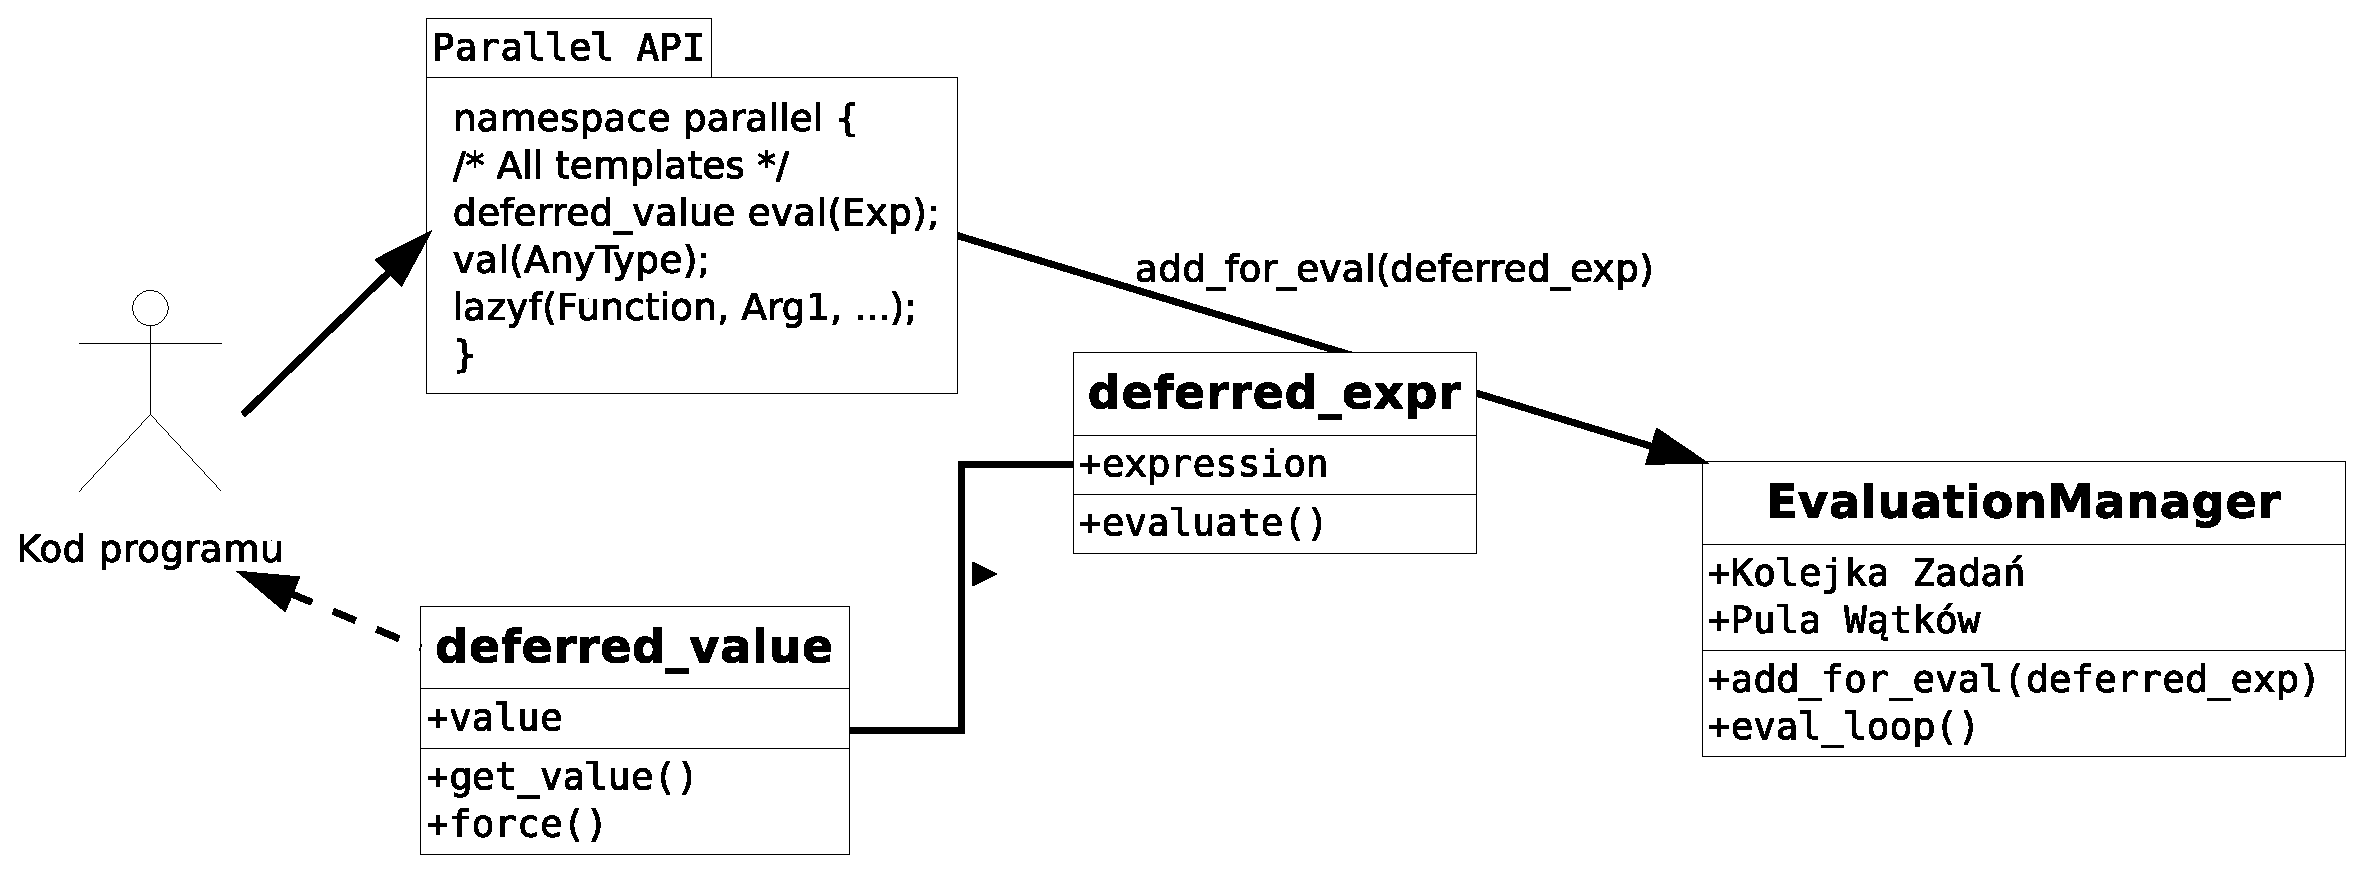
\includegraphics[width=\textwidth]{architecture.eps}
 \caption{Schemat architektury biblioteki Parallel}
\end{figure}

  Diagram przedstawia najwa�niejsze elementy statycznej struktury biblioteki wraz z zale�no�ciami mi�dzy nimi.
  Na diagramie nie znajduj� si� wszystkie metody zaimplementowane w poszczeg�lnych klasach, a jedynie te niezb�dne do zaprezenowania sposobu architektury biblioteki.
  
\subsection{API biblioteki}

  Kod programu komunikuje si� z bibliotek� poprzez API. Oto kr�tkie wyja�nienie znaczenia poszczeg�lnych funkcji z API:
  G��wn� funkcj� z API jest funkcja \feval, kt�rej znaczenie zosta�o opisane w sekcji \nameref{sss:eval}.
  Pozosta�e funkcje maj� zadanie pomocnicze w stosunku do \feval.
  S� niezb�dne do stworzenia wyra�enia, kt�re funkcja \feval mo�e przyj�� do wyliczenia.
  I tak odpowiednio funkcja \verb|val| pozwala przekaza� sw�j argument do wyra�enia przez warto��, \verb|cval| przez warto�� sta��, \verb|ref| przez referencj�, \verb|cref| przez sta�� referencj�.
  Ponadto w API znajduje sie wzorzec funkcji pozwalaj�cy na uleniwione wywo�ywanie funkcji, \verb|lazyf|.
  Dok�adna rola i spos�b tych funkcji jest opisana w sekcji \nameref{s:przekazywanie_wyrazen}.
  Nale�y doda�, i� program korzystaj�cy z biblioteki Parallel musi przed rozpocz�ciem zlecania wyra�e� do obliczenia wywo�a� funkcj� \verb|init|
  inicjalizuj�c� bibliotek� i ustalaj�c� liczb� w�tk�w w puli mechanizmu ewaluacji.
  Korzystanie z biblioteki Parallel powinno zako�czy� si� wywo�aniem funkcji \verb|close|, kt�ra zwalnia zasoby zaalokowane przez bibliotek�.
  
\subsection{Operacje wykonywane w kodzie biblioteki Parallel}\label{ss:operacje}

  Odpowiednio stworzone wyra�enie jest przetwarzane przez funkcj� \feval.
  W ciele funkcji z wyra�enia tworzony jest obiekt typu \verb|deferred_expr| z przypisanym odpowiednim wyra�eniem, kt�ry reprezentuje zadanie do wykonania.
  Zadanie do wykonania jest dodawane do kolejki zada� w obiekcie \emgr przy u�yciu metody \verb|add_for_eval|.
  Aparat wykonawczy w postaci instancji typu \emgr zawiera opr�cz kolejki zada� do wykonania r�wnie� w�tki, kt�rymi zarzadza i kt�re te zadania wykonuj� dzia�aj�c w niesko�czonej p�tli w funkcji \verb|eval_loop|.
  Ka�dy obiekt typu \verb|deferred_expr| jest po��czony 1-1 z obiektem typu \dval, kt�ry reprezentuje wynik obliczenia wyra�enia.
  Je�li zadanie zdefinowane przez wyra�enie zapisane w obiekcie \dexp zostaje wykonane, to wynik (je�li istnieje) zostaje przypisany na pole \verb|value| w skojarzonym obiekcie typu \dval.
  
\subsection{Zwr�cenie wyniku}
  
  Wynik jest przekazywany do kodu programu poprzez warto�� typu \verb|deferred_value|, kt�ra jest zwracana jako wynik funkcji \feval.
  Je�li nast�pi wywo�anie pobrania warto�ci z obiektu typu \dval metod� \verb|get_value| lub wymuszenie wyliczenia warto�ci przez metod� \verb|force| to je�li skojarzone \dexp nie zosta�o wykonane
  to wyliczenie wyra�enia zostanie wymuszone, o ile si� jeszcze nie rozpocz�o.
  
  
\section{Implementacja przekazywania wyra�e� do wyliczenia}\label{s:przekazywanie_wyrazen}
  
  Zaprojektowanie przekazywania wyra�e� do wykonania by�o jednym z najtrudniejszych zada� podczas fazy implementacji biblioteki Parallel.
  Mechanizm mia� stanowi� wa�n� cz�� API biblioteki, kt�re powinno wspiera� spe�nienie wyznaczonych dla biblioteki cel�w czytelno�ci i intuicyjno�ci.
  Te cele niew�tpliwie by�yby zrealizowane, gdyby mo�liwe by�o przekazywanie wyra�e� w ich standardowej postaci w j�zyku C++.
  Jednak problem stanowi� fakt, i� j�zyk C++ posiada gorliw� semantyk� wyliczania wyra�e�.
  Definicja problemu podpowiada�a rozwi�zanie, skoro problemem jest gorliwo�� nale�a�o wyra�enia przekazywane do wyliczenia uleniwi�.
  
  Najbardziej naturalne by�oby u�ycie s�owa kluczowego lub funkcji, kt�ra uleniwia�aby wyra�enie.
  Pierwszy pomys� by� nie do zrealizowania, poniewa� j�zyka C++ nie mo�na rozszerzy� o nowe s�owa kluczowe, a standard j�zyka nie przewidzia� s�owa kluczowego dla uleniwiania wyra�e�.
  Uleniwienie poprzez u�ycie funkcji mog�oby wygl�da� nast�puj�co:
  \begin{lstlisting}[numbers=none,frame=none]
   make_lazy_expression(4 + fibonacci(20));
  \end{lstlisting}
  Jednak semantyka j�zyka C++ r�wnie� nie pozwala�a na tak� realizacj� uleniwiania wyra�e�, gdy� wyra�enie podane jako argument jest wyliczane przed wywo�aniem funkcji.
  
  Metoda rozwi�zania problemu uleniwiania wyra�e� okaza�a si� by� bardziej skomplikowana i zosta�a zainspirowana przez idiom C++ szablonu wyra�enia,
  kt�ry jako jedna z dobrych praktyk j�zyka C++ zosta� opisany w ksi��ce \textit{More C++ Idioms} \cite{idioms}.
  Implementacja tego szablonu nie by�aby mo�liwa gdyby nie bardzo silny szablon�w typ�w i funkcji w j�zyku C++.

\subsection{Szablony w j�zyku C++}

  Nie chcia�bym zamieszcza� tutaj opisu podstawowych informacji na temat szablon�w.
  Wprowadzenie do tej tematyki mozna przeczyta� w ksi��ce \cite{c++lang}.
  Moim celem jest pokazanie, dlaczego implementacja przekazywania wyra�e� tak jak tego dokona�em by�a mo�liwa.
  
  Szablony s� bardzo silnym mechanizmem, aczkolwiek si�a ekspresyjna szablon�w nie by�a zamierzona przez tw�rc�w i dopiero przypadkiem zosta�y odkryte mo�liwo�ci, kt�re daj�.
  Szablony C++ s� w rzeczywisto�ci pewnym funkcyjnym j�zykiem programowania o ekspresywno�ci rachunku lambda.
  Udowodniono, i� mechanizm szablon�w jest r�wnowa�ny maszynie Turinga (\cite{turingcom}).
  W praktyce oznacza to tyle, �e szablony C++ pozwalaj� dokonywac dowolnych oblicze� w oparciu o typy.
  Oto przyk�ad obliczania silni w czasie kompilacji przy pomocy szablon�w:
  \begin{lstlisting}
template< unsigned n >
struct factorial {
  static const unsigned value = 
    n * factorial<n-1>::value;};
template<>
struct factorial<0> {
  static const unsigned value = 1; };
  \end{lstlisting}
  Obliczenie odbywa si� rekurencyjnie, granic� rekurencji jest \verb|factorial<0>|, kt�re jest specjalizacj� szablonu \verb|factorial|.
  Taka konstrukcja pozwala obliczy� dowolne warto�ci silni w czasie kompilacji
  \footnote{Pewnym ograniczeniem jest limit kompilatora na rekurencyjne konkretyzowanie szablon�w, ale ten limit mo�na zmieni� przy pomocy odpowiednich opcji} i korzysta� z nich w czasie sta�ym podczas wykonania programu.
  
\subsection{Idiom C++ szablonu wyra�enia}

  Intuicyjnie rzecz ujmuj�c, idiom szablonu wyra�enia polegana opisaniu wyra�enia przy pomocy instancji pewnego szablonu typu.
  Ten typ nie jest nigdy zapisywany w postaci jawnej w programie, gdy� nale�a�oby oczekiwa�, �e sk�adnia szablonu typu by�aby wtedy bardzo nieczytelna.
  Zamiast tego szablon typu jest tworzony w wyniku oblicze� na typach udost�pnianych przez mechanizm rozwijania szablon�w w j�zyku C++.
  Idiom szablonu wyra�enia wykorzystuje inny idiom Rekurencyjnego Sk�adania Typ�w (z ang. Recursive Type Composition). 
  Polega on na tym, �e szablon typu zawiera pola, kt�rych typem jest jest instancja tego samego szablonu typ�w.
  W tym przypadku szablon wyra�enia mo�e zawiera� pola, kt�re s� szablonem wyra�enia.
  W ten spos�b powstaje drzewo reprezentuj�ce wyra�enie w postaci drzewa typ�w. 
  Taka konstrukcja nazywana jest Abstrakcyjnym Drzewem Syntaktycznym (z ang. Abstract Syntax Tree - AST).
  W takiej konstrukcji w li�ciach drzewa znajduj� si� terminale wyra�enia, czyli szablony wyra�enia nie zawieraj�ce ju� w sobie �adnych szablon�w wyra�enia.
  Natomiast w w�z�ach po�rednich reprezentowane s� operatory u�yte w wyra�eniu, kt�re jako pola posiadaj� szablony wyra�enia, b�d�ce argumentami operatora.
  Ka�demu operatorowi odpowiada reprezentuj�cy go szablon typu, z odpowiednio zaimplementowan� funkcj� aplikuj�c� operator, w momencie, gdy szablon wyra�enia jest wyliczany.
  
  Zaprezentuj� ide� szablonu wyra�enia na przyk�adzie, w kt�rym jedyn� dozwolon� operacj� b�dzie dodawanie liczb ca�kowitych lub zmiennoprzecinkowych.
\begin{lstlisting}
/*** TYPY ODPOWIEDZIALNE ZA BUDOW� DRZEWA AST ***/

template <typename T> struct Exp;

template <typename T>
struct Term : Exp<Term<T> >
{
  Term(T v) : val(v){}
  const T val;
};

/* Definicje wez��w reprezentuj�cych operatory */

template <typename T1, typename T2>
struct Sum : Exp<Sum<T1, T2> >
{
  Sum (T1 l, T2 r) : lhs(l), rhs(r) {}
  const T1 lhs;
  const T2 rhs;
};

template <typename T1, typename T2>
struct Mul: Exp<Mul<T1, T2> >
{
  Mul(T1 l, T2 r) : lhs(l), rhs(r) {}
  const T1 lhs;
  const T2 rhs;
};

/* Wzorzec Infer s�u�y do obliczania typu wynikowego wyra�enia */

template <typename E> 
struct Infer {
  typedef E type ; 
};

template <typename T>
struct Infer<Term<T> >
{
  typedef T type;
};

/* Wnioskowanie dla sumy zgodnie z semantyk� j�zyka C++ */

template < >
struct Infer< Sum<double,double> > 
{ 
  typedef double type; 
};

template < >
struct Infer< Sum<double,int> > 
{
  typedef double type;
};

template < > 
struct Infer< Sum<int,double> > 
{
  typedef double type; 
};

template < > 
struct Infer< Sum<int,int> > 
{ 
  typedef int    type;
};

/* Typ(T1 + T2) to typ sumy(typ(T1),typ(T2)) */
template <typename T1, typename T2> 
struct Infer < Sum<T1,T2> > {
  typename Infer<T1>::type typedef T1T ;
  typename Infer<T2>::type typedef T2T ;
  typename Infer<Sum<T1T,T2T> >::type typedef type;
} ;

/* Wnioskowanie o typach dla wzorca Mul jest analogiczne */

/* Wzorzec Exp umo�liwia unikni�cie definicji operator�w
 * w ka�dym typie reprezentujacym weze� po�redni w drzewie AST */
 
template <typename T>
struct Exp
{
  template <typename U>
  inline Sum<T,U> operator + (U u) 
  { 
    /* static_cast jest potrzebny i prawid�owy, 
     * poniewa� Exp jedynie obudowuje typ T */
    return Sum<T,U>(static_cast<T>(*this), u); 
  }
  
  template <typename U>
  inline Mul<T,U> operator * (U u)
  {
    return Mul<T,U>(static_cast<T>(*this), u);
  }
};

template <typename T, typename U>
Sum<T,U> operator + (T t, Exp<U> u)
{
  return Sum<T,U>(t, static_cast<U>(u));
}

template <typename T, typename U>
Mul<T,U> operator * (T t, Exp<U> u)
{
  return Mul<T,U>(t, static_cast<U>(u));
}

/*** DEFINICJE FUNKCJI EWALUUJ�CYCH DRZEWA AST ***/

inline template <typename T>
Infer<T>::type eval(Exp<T> exp)
{
  return eval(static_cast<T>(exp));
}

inline template <typename T>
Infer<Term<T> >::type eval(Term<T> term)
{
  return term.val;
}

inline template <typename T1, typename T2>
Infer<Sum<T1, T2> >::type eval(Sum<T1, T2> sum)
{
  return eval(sum.lhs) + eval(sum.rhs);
}

inline template <typename T1, typename T2>
Infer<Mul<T1, T2> >::type eval(Mul<T1, T2> mul)
{
  return eval(mul.lhs) + eval(sum.rhs);
}

/* Potrzebna jest tak�e definicja int eval (int) 
 * oraz double eval(double), poniewa� nie ma wymogu,
 * aby zawsze te typy proste by�y obudowane w Term. */
 
inline int eval(int i) {return i;}
inline double eval(double d) {return d;}
\end{lstlisting}

  Wzorzec \verb|Term| (linie 6-11) umo�liwia oznaczenie dowolnej warto�ci jako li�cia w drzewie reprezentujacym szablon wyra�enia.  
  Teoretycznie wszystkie warto�ci powinny byc oznaczone w ten spos�b.
  Jednak jak sie p�niej dowiemy identyczne dzia�anie mo�na uzyska� oznaczaj�c tylko cz�� warto�ci.
  
  Wzorce \verb|Sum| oraz \verb|Mul| reprezentuj� wez�y po�rednie w drzewie AST (linie 15-29).
  Ich lewa i prawa strona reprezentuj� odpowiednie podwyra�enia, b�d�ce argumentami operatora binarnego.
  Najciekawszym zabiegiem u�ytym w ich definicji jest podanie definicji tego� samego wzorca jako argumentu wzorca Exp, b�d�cego klas� bazow� wzorc�w operator�w.
  Ma to miejsce przyk�adowo w tym fragmencie kodu: \verb|struct Sum : Exp<Sum<T1, T2> >| i jest w pe�ni dozwolone przez sk�adni� j�zyka.
  Dzi�ki takiemu zabiegowi mo�na poda� implementacj� operator�w tylko we wzorcu \verb|Exp|, a nie jest to konieczne we wszystkich innych wzorcach w�z��w po�rednich.
  \verb|Sum<T1, T2>| dziedziczy metody przedefiniuj�ce operatory, z tym, �e te definicje s� dopasowane do \verb|Sum<T1, T2>|, poniewa� s� parametryzowane tym typem.
  
  Kolejna cz�� przyk�adu (linie 33-78) zajmuje si� definicj� wzorca \verb|Infer|, kt�ry oblicza typ wynikowy wyliczenia wyra�enia, b�dzie on potrzebny do definicji funkcji ewaluuj�cych wyra�enie.
  Wykorzystywany jest tutaj mechanizm specjalizacji wzorc�w w j�zyku C++, kt�ry pozwala okre�li� typ wynikowy wyra�enia w zale�no�ci od postaci wzorca.
  Og�lnie, podczas definicji wnioskowania o typach nale�y pami�ta� o uwzgl�dnieniu wszystkich istotnych specjalizacji wzorca, czyli dla w�z��w po�rednich jak \verb|Term|, \verb|Sum|, \verb|Mul|
  oraz wszystkich mo�liwych typ�w, kt�re mog� wystapi� w w�z�ach po�rednich.
  Jak wida� implementacja szablonu wzorca wnioskuj�cego o typie wynikowym wyra�enia jest bardzo d�uga i czasoch�onna (do tego stopnia, �e pomin��em cz�� po�wi�con� wnioskowaniu typu dlaczego
  wzorca \verb|Mul|, gdy� jest ona dok�adnie analogiczna jak cz�� dotycz�ca wzorca \verb|Sum|.
  
  Na koniec sekcji kodu, kt�ra tworzy AST (linie 83-99) znajduje si� definicja wzorca \verb|Exp|, kt�rego rola zosta�a opisana powy�ej.
  \verb|Exp| uwsp�lnia definicje operator�w w klasach w�z��w po�rednich.
  
  Kolejna du�a sekcja kodu przyk�adu (linie od 103 do 132) definiuje funkcj� \feval, kt�ra s�u�y do obliczania warto�ci szablonu wyra�enia.
  Funkcja \feval przyjmuje jako argument szablon wyra�enia (albo warto�� prost� int lub double), a nast�pnie oblicza jego warto�� zgodnie z semantyk� j�zyka C++.
  Typ zwracamy przez \feval jest obliczany przy pomocy wzorca \verb|Infer|.
  
\subsubsection{Szablon wyra�enia w dzia�aniu}
  Zrozumienie kodu szablonu wyra�enia przedstawionego powy�ej b�dzie �atwiejsze po przeanalizowaniu przyk�ad�w jego dzia�ania.
  We�my najprostszy mo�liwy przyk�ad:
  \begin{lstlisting}[numbers=none, frame=none]
   Term(4) + Term(5);
  \end{lstlisting}
  Wyra�enie reprezentuje dodanie dw�ch liczb ca�kowitych i szablon wyra�enia, kt�ry zostanie stworzony w wyniku oblicze� na typach b�dzie wygl�da� nast�puj�co:
  \begin{lstlisting}[numbers=none, frame=none]
   Sum<Term<int>,Term<int> >
  \end{lstlisting}
  Ju� na bazie tego prostego przyk�adu nasuwa si� kilka ciekawych kwestii do om�wienia.
  
  Po pierwsze mo�na si� zastanowi�, po co sk�adania jest tak przegadana oraz czy potrzebne jest pisanie \verb|Term| przy ka�dej warto�ci przekazywanej do wyra�enia.
  Wiadomo na pewno, �e co najmniej jedna warto�� musi by� oznaczona jako terminal szablonu wyra�enia.
  Jest tak, poniewa� je�li, �adna z warto�ci nie by�aby oznaczona by�oby to zwyk�e wyra�enie C++ i zosta�oby obliczone gorliwie.
  Ponadto, nie da si� tego zmieni� przy pomocy przeci��ania operator�w, gdy� co najmniej jednym argumentem operatora musi by� klasa lub typ wyliczeniowy.
  Zastan�wmy si�, czy poni�sze wyra�enie jest poprawne sk�adniowo i je�li tak, to jaki b�dzie szablon typu, kt�ry powstanie.
  \begin{lstlisting}[numbers=none, frame=none]
   Term(4) + 5;
  \end{lstlisting}
  W tym wyra�eniu mamy do czynienia z operacj� dodawania typu \verb|Term<int>| oraz typu \verb|int|.
  Poniewa� \verb|Term<int>| dziedziczy operator dodawania z \verb|Exp<Term<int> >| to zostanie wywo�any operator dodawania zdefinowany w linii 87 przyk�adu.
  Warto zauwa�y�, �e typ prawego argumentu nie jest w �aden spos�b ograniczony, wi�c zastosowanie typu int jest poprawne i podane wyra�enie jest poprawne sk�adniowo.
  W zwi�zku z tym wynikiem budowy drzewa tego wyra�enia b�dzie \verb|Sum<Term<int>, int>|.
  To pokazuje, �e szablon wyra�enia zostanie zbudowany poprawnie r�wnie� wtedy, gdy nie wszystkie warto�ci zostan� oznaczone jako terminale.
  Jednak�e, cz�� warto�ci, a co najmniej jedna musi zosta� oznaczona, gdy� inaczej budowa szablonu wyra�enia nie zostanie zapocz�tkowana i wyra�enie nie zostanie uleniwione, a obliczy si� normalnie.
  
  Wa�nym faktem jest to, �e budowa drzewa AST ma miejsce w czasie kompilacji, wi�c budowanie szablon�w wyra�e� nie nak�ada narzut�w na czas wykonania programu.
  Natomiast narzuty podczas ewaluacji uleniwionego wyra�enia zale�� od tego w jakim stopniu kompilator zoptymalizowa� wywo�ania funkcji \feval wyliczaj�cej warto�� wyra�enia poprzez jej rekurencyjne rozwini�cie w miejscu wykonania.
  W najgorszym przypadku nast�pi jedno wywo�anie funkcji dla ka�dego w�z�a po�redniego.
  
  Teraz na bardziej zaawansowanym przyk�adzie zbadamy to jakie s� zasady decyduj�ce o tym kiedy dodanie oznaczenia \verb|Term| jest wymagane, aby uleniwienie wyra�enia dzia�a�o zgodnie z �yczeniem programisty.
  Do tej analizy pos�u�� dwa poni�sze przyk�ady uleniwionych wyra�e�:
  \begin{lstlisting}[frame=none, numbers=none]
   4 + 5 * Term(6); /* (1) */
   
   Term(4) + 5 * 6; /* (2) */
  \end{lstlisting}
  Nale�y mie� �wiadomo��, �e du�� rol� w procesie budowy drzewa AST odgrywaj� priorytety operator�w.
  To one decyduj� w du�ej mierze o postaci drzewa i o tym w jaki spos�b wyra�enie zostanie uleniwione.
  
  W pierwszym wyra�eniu najpierw kompilator zajmie si� podwyra�eniem \verb|5 * Term(6)|, kt�re da w rezultacie \verb|Mul<int, Term<int> >|.
  Warto odnotowa�, �e tym razem tylko prawy argument operatora binernego by� typem szablonu wyra�enia, wi�c zosta� u�yty operator zdefinowany w linii 108 przyk�adu.
  W nastepnej kolejno�ci nast�pi dodawanie 4 oraz wyra�enia typu \verb|Mul<int, Term<int> >|, co da w wyniku kolejny bardziej rozbudowany szablon wyra�enia \verb|Sum<int, Mul<int, Term<int> > >|.
  Uda�o si� pokaza�, �e pierwsze z analizowanych wyra�e� zachowa si� zgodnie z intencj� programisty, to znaczy ca�e wyra�enie zostanie uleniwione.
  
  Analogicznie badamy zachowanie wyra�enia drugiego.
  Na pocz�tku spostrzegamy, �e najpierw dojdzie do obliczenia podwyra�enia \verb|5 * 6|. 
  Zatem ewaluacja odb�dzie si� gorliwie, poniewa� budowa szablonu wyra�enia nie zosta�a zapocz�tkowana, mamy tu do czynienia ze zwyk�ym mno�eniem.
  W nast�pnym kroku odb�dzie si� dodawanie \verb|Term(4)| i wyniku \verb|5 * 6|, czyli \verb|30|, czego konsekwencj� b�dzie stworzenie szablonu wyra�enia \verb|Sum<Term<int>, int>|.
  To nie jest to czego oczekiwali�my, gdy� za�o�yli�my, �e chcemy uleniwi� ca�e wyra�enie, a zasz�o to jedynie dla jego cz�ci.
  
  Wnioskiem z powy�szej analizy jest to w jaki spos�b dochodzi do propagowania si� leniwo�ci w czasie budowania szablonu wyra�enia.
  To propagowanie zachodzi od warto�ci oznaczonej jako terminal w g�r� drzewa.
  St�d ka�dy operator na �cie�ce pomi�dzy uleniwionym terminalem, a korzeniem drzewa (w��cznie) b�dzie uleniwiony, czyli nie b�dzie wywo�any od razu, 
  a zostanie zakodowany w strukturze szablonu wyra�enia i wywo�any, gdy nast�pi wymuszenie obliczenia wyra�enia.
  W szczeg�lno�ci, pisz�c kod tworz�cy szablony wyra�enia w oparciu o przedstawiony przyk�ad nale�y mie� na uwadze to, �e tworzenie drzew AST przez kompilator nie jest jednoznaczne,
  poniwa� kompilator mo�e w przypadku wyst�pienia obok siebie operator�w o identycznym priorytecie stworzy� r�ne drzewa AST.
  Przyk�adem jest wyra�enie \verb|4 + 5 + 6|.
  
\subsection{Praktyczna implementacja szablonu wyra�enia -- Boost.Proto}

  Przedstawiony powy�ej spos�b da si� uog�lni� dla dowolnego wyra�enia w j�zyku C++.
  To znaczy, �e stworzenie dowolnego leniwego wyra�enia jest mo�liwe, do czego d��y�em podczas pisania pracy.
  Jednak�e napisanie takiej biblioteki od podstaw wykracza�o poza ramy tej pracy magisterskiej.
  Dlatego si�gn��em po rozwi�zania ju� istniej�ce, publicznie dostepne.
  Wybra�em bibliotek� Boost.Proto w celu implementacji uleniwionych wyra�e�, metod� szablon�w wyra�e�.
  
  Boost.Proto jest bibliotek� s�u��c� do tworzenia Wbudowanych J�zyk�w Domenowych (z ang. Domain Specific Embedded Language) w j�zyku C++. 
  Zawiera narz�dzia do tworzenia, sprawdzania typ�w, przetwarzania oraz wykonywania szablon�w wyra�e�. Proto zapewnia:
  \begin{itemize}
   \item Szablony wyra�e� w postaci AST
   \item Mechanizm modyfikacji zachowania wyra�e�
   \item Przeci��anie operator�w dla budowy AST z wyra�enia
   \item Narz�dzia do definiowania gramatyki wyra�e�
   \item Rozszerzalny mechanizm natychmiastowego wyliczenia szablonu wyra�enia
   \item Rozszerzalny zestaw operacji przetwarzania na szablonach wyra�e�
  \end{itemize}

  Biblioteka Boost.Proto zosta�a wykorzystana do implementacji nast�puj�cych komponent�w biblioteki Parallel:
  \begin{itemize}
   \item Funkcje do oznaczania terminali:
   \begin{itemize}
    \item \verb|val| -- funkcja przekazuj�ca terminal do wyra�enia przez warto��
    \item \verb|cval| -- funkcja przekazuj�ca terminal do wyra�enie przez sta�� warto�� (modyfikator \verb|const|)
    \item \verb|ref| -- funkcja przekazuj�ca terminal do wyra�enia przez referencj�
    \item \verb|cref| -- funkcja przekazuj�ca terminal do wyra�enia przez sta�� referencj�
   \end{itemize}
   \item \verb|lazyf| -- funkcja s�u��ca do tworzenia uleniwionego wywo�ania funkcji
   \item \verb|deferred_expr| -- szablon typu przechowuj�cego uleniwione wyra�enia i zarz�dzaj�cego jego wyliczeniem
  \end{itemize}
  
  Biblioteka Parallel korzysta z Boost.Proto do tworzenia szablon�w wyra�e� w postaci AST, r�wnie� przy pomocy mechanizmu przeci��ania operator�w, dzi�ki czemu budowa AST jest uproszczona.
  Ponadto ewaluacja odbywa si� przy pomocy dostarczonej przez Boost.Proto funkcji \verb|proto::eval| z domy�lnym zachowaniem.
  Zasada dzia�ania Boost.Proto jest analogiczna do dzia�ania przyk�adu pokazanego powy�ej.

\subsection{Alternatywne rozwi�zanie}

  Do wyboru by�a r�wnie� inna mo�liwo�� realizacji przekazywania wyra�enia ni� forma uleniwiona opisana to powy�ej.
  Podobny efekt mo�na uzyska� stosuj�c obiekty funkcyjne, kt�re reprezentowa�yby dane wyra�enie.
  Istnieje jednak istotny pow�d, dla kt�rego zosta�o wybrane pierwsze z przedstawionych rozwi�za�.
  Leniwe wyra�enia maj� bardziej intuicyjn� sk�adni�, natomiast tworzenie odpowiednich obiekt�w funkcyjnych wymaga znajomo�ci stosownych bibliotek.
  Przyk�adami s� Boost.Lambda, Boost.Function i Boost.Bind, jednak�e pomimo tego, �e s� to jedne z najlepszych bibliotek w swojej klasie ich sk�adnia jest w przypadku pisania rozbudowanego wyra�enia zdecydowanie nieintuicyjna.
  Szczeg�lnie problematyczny jest zapis zagnie�d�onych funkcji, w tym operator�w.
  Nast�puj�cy kawa�ek kodu nie nale�y do czytelnych:
\begin{verbatim}
  bind(f, bind(operator+,5,4)); //f(5+4)
\end{verbatim}
  Zamiast bardziej intuicyjnego:
\begin{verbatim}
  fun(f)( val(5) + val(4) );
\end{verbatim}
  Tak naprawd� wystarczy�oby
\begin{verbatim}
 f(val(5)+4);
\end{verbatim}
  gdy� \verb|val(5)| wprowadzi�oby leniwo�� na najni�szym poziomie w drzewie wyra�enia, kt�ra nast�pnie propagowa�aby si� w stron� potomk�w i rodze�stwa tego w�z�a w drzewie wyra�enia.

  St�d ze wzgl�du na znacznie bardziej intuicyjn� sk�adni� dla przekazywania oblicze� do wykonania r�wnoleg�ego zosta�y wybrane leniwe wyra�enia.

\section{Implementacja mechanizmu ewaluacji}\label{s:ewaluacja}

  Zarys mechanizmu ewaluacji zosta� przedstawiony w sekcji \nameref{ss:wykonywanie}.
  G��wn� funkcj� mechanizmu ewaluacji jest pobieranie zada� (wyra�e� do obliczenia) zlecanych przez kod programu i ich ewaluacja.
  Do implementacji tej cz�ci biblioteki wykorzystano wzorzec projektowy puli w�tk�w oraz kolejki zada�.
  G��wn� klas� tej cz�ci biblioteki jest \verb|evaluation_mgr| (od ang. evaluation manager -- mened�er ewaluacji), kt�ra jest singletonem i zarz�dza ca�o�ci� procesu wykonywania zada�.
  
\subsection{Zadania w bibliotece Parallel}

  Zadaniem w kontekscie biblioteki Parallel nazywam uleniwione wyra�enie, kt�re zosta�o przekazane bibliotece do obliczenia.
  Zadanie jest reprezentowane przez wzorzec typu \verb|deferred_expr| (od ang. deferred expression -- wyra�enie odroczone).
  Naistotniejsz� w�asno�cia \verb|deferred_expr| jest to, �e jedyny konstruktor publiczny przyjmuje jako argument szablon wyra�enia, taki jaki zosta� opisany w sekcji \nameref{s:przekazywanie_wyrazen}.
  Szablon wyra�enia jest przechowywany jako jedno z p�l \verb|deferred_expr|.
  Ten szablon wyra�enia jest poddawany ewaluacji po wywo�aniu metody \verb|evaluate|.
  Pozosta�e pola i metody \verb|deferred_expr| s�u�a kontrolowaniu wyliczenia wyra�enia oraz przekazywaniem wyniku do skojarzonego obiektu typu \verb|deferred_value|
  \footnote{Zgodnie z opisem z \nameref{ss:operacje} obiekt \dexp jest skojarzony 1-1 z obiektem \dval.}.
  
\subsection{Pula w�tk�w}

  Wzorzec puli w�tk� zosta� wybrany ze wzgl�du na efektywno��.
  Dzi�ki takiej implementacji unika si� tworzenia w�tku dla ka�dego zadania do wykonania, co jest operacj� dosy� drog� i warto zadba�, aby nie by�a wykonywana zbyt cz�sto.
  Ka�dy z w�tk�w dzia�a w niesko�czonej p�tli w funkcji \verb|eval_loop|, w kt�rej w�tek pr�buje pobra� zadanie do wykonania z kolejki zada�, a je�li nie jest ono dost�pne to czeka na zmiennej warunkowej.
  Do implementacji zosta�a wykorzystana biblioteka Boost.Threads.
  
  Pula w�tk�w pozwala w �atwy spos�b unikn�� innego problemu zwi�zanego z tworzeniem w�tku dla ka�dego zadania.
  W przypadku gdyby pojawi�o si� zbyt wiele zada� jednocze�nie liczba w�tk�w mog�aby wzrosn�� do takiej liczby, �e wydajno�� programu znacznie by spad�a z powodu cz�stego prze��czania kontekstu pomi�dzy r�nymi w�tkami.
  Pula w�tk�w pozwala ustali� maksymaln� liczb� w�tk�w, wi�c pewna liczba nigdy nie zostanie przekroczona i je�li zostanie ustawiona odpowiedno, nie dojdzie przeci��enia systemu.
  Obecnie liczba w�tk�w jest ustalana przez programist�, nic nie stoi na przeszkodzie, aby w przysz�o�ci liczba w�tk�w by�a dobierana automatycznie w zale�no�ci od wydajno�ci systemu b�d� innych parametr�w.
  
\subsection{Kolejka zada�}

  Kolejka zada� jest standardow� kolejk� FIFO przechowuj�c� obiekty \dexp.
  Poniewa� jednocze�nie kod programu lub ka�dy z w�tk�w z puli przechowywanej w \verb|evaluation_mgr| mo�e chcie� skorzysta� z kolejki, dost�p do niej jest chroniony sekcj� krytyczn�.
  Dodawanie zada� do kolejki odbywa si� w ciele funkcji \feval przy u�yciu funkcji \verb|add_for_eval|.

\subsection{Procedura ewaluacji}

  Procedura ewaluacji z punktu widzenia mechanizmu ewaluacji wygl�da bardzo prosto.
  W�tek-robotnik pobrawszy zadanie wywo�uje jego metod� \verb|evaluate|.
  To skutkuje wyliczeniem wyra�enia, a je�li typ wynikowy wyra�enie jest inny ni� \verb|void| to warto�� zostaje przekazana do skojarzonego obiektu \dval.
  Po wyliczeniu wyra�enia obiekt \dexp jest niszczony, gdy� nie jest ju� potrzebny.
  
  Ten obraz komplikuje si�, gdy rozwa�ymy pewien bardzo istotny scenariusz.
  Ot� nie ma problemu je�li, w�tki-robotnicy nad��aj� z ewaluacja z zada� z kolejki.
  Jednak, gdy d�ugo�� kolejki wzro�nie mo�e dojs� do sytuacji, �e w�tek programu, kt�ry zleci� wyliczenie wyra�enia b�dzie potrzebowa� jego warto�ci.
  Wtedy nast�pi pr�ba pobrania warto�ci z obiektu \dval, kt�ry jeszcze nie otrzyma� obliczonej warto�ci.
  To oznacza, �e w�tek programu musi zawiesi� wykonywanie i poczeka�, a� warto�� zostanie obliczona.
  
  Nie jest z�� sytuacj�, gdy w�tek programu oczekuje, gdy ewaluacja wyra�enia ju� si� rozpocz�a, poniewa� warto�� zostanie przekazana tak szybko jak to mo�liwe.
  Jednak, gdy zadanie, na kt�re kod programu oczekuje, jeszcze nie zosta�o pobrane do wykonania dochodzi do absurdalnej sytuacji, 
  dlatego, �e w�tek programu nic nie robi i czeka na wykonanie zadania, podczas gdy m�g�by sam wykona� potrzebne obliczenia.
  Odpowienio zaimplementowana procedura ewaluacji w bibliotece Parallel unika tego problemu.
  
  W analogicznej sytuacji w�tek programu, gdy zorientuje si�, �e wyra�enie nie zosta�o obliczone sam dokona ewaluacji.
  Zostanie wywo�ana ta sama procedura \verb|evaluate|, kt�r� wywo�uj� w�tki-robotnicy.
  Mo�e to skutkowa� zdublowanym wyliczeniem wyra�enia, w przypadku, gdy zar�wno w�tek programu, jak i jeden z w�tk�w-robotnik�w obliczyliby wyra�enie.
  Taka sytuacja by�aby niedopuszczalna, poniewa� obliczanie w C++ nie jest idempotentne z powodu efekt�w ubocznych.
  
  Najbardziej standardowym rozwi�zaniem by�oby umieszczenie w ka�dym obiekcie \dexp flagi wraz mutex-em j� chroni�cym w celu zapobie�enia podw�jnej ewaluacji wyra�enia.
  Zapewni�oby to r�wnie� drobn� ziarnosto�� ochrony, co zwi�ksza�oby wsp�bie�no�� i jednocze�nie wydajno�� dzia�ania biblioteki.
  Jednak�e umieszczenie mutex-a w ka�dym obiekcie ma pewien narzut pami�ciowy i wydajno�ciowy.
  
  Na szcz�cie istnieje lepsze rozwi�zanie tego problemu mo�liwe dzi�ki funkcji z biblioteki Boost Threads \verb|call_once| gwarantuj�cej jednokrotne wywo�anie funkcji.
  Przekazanie tej funkcji zmiennej typu \verb|once_flag| wraz z funkcj� do wykonania (w tym przypadku funkcj� \verb|deferred_expr::evaluate|) sprawi, �e dla danej flagi funkcja wykona si� tylko raz.
  Wywo�anie \verb|call_once| z innego w�tku lub ponownie z tego samego z ju� raz wykorzystan� flag� \verb|once_flag| zako�czy si� natychmiast bez wywo�ania przekazanej funkcji.
  Poniewa� typ \verb|once_flag| ma niewielki rozmiar (na wi�kszo�ci platform jest to typ \verb|long|) to umieszczenie go jako pola ka�dego obiektu \dexp dodaje mniejszy narzut pami�ciowy ni� stosowanie mutex-�w.
  
  Innym wa�nym aspektem procedury ewaluacji odroczonego wyra�enia jest obs�uga wyj�tk�w.
  Zgodnie z koncepcj� biblioteki wyj�tki, kt�re wyst�pi� podczas ewaluacji wyra�enia (w ciele funkcji \verb|evaluate| s� wywo�ywane, a nast�pnie przekazywane do obiektu \dval zamiast wyniku.
  Dzi�ki temu wyj�tek b�dzie m�g� zosta� przekazany z obiektu \dval do g��wnego w�tku programu.
  
\subsection{Ograniczenia mechanizmu ewaluacji}

  W zwi�zku ze sposobem przekazywania wyra�e� do obliczenia, mo�liwo�ci projektowania mechanizmu ewaluacji by�y do�� powa�nie ograniczone.
  W og�lno�ci mogliby�my wyobrazi� sobie sytuacj�, w kt�rej wyra�enie z programu dzia�aj�cego na jednym komputerze by�oby przekazywane do wyliczenia do innych program�w lub nawet do innych komputer�w, w celu wi�kszego rozproszenia i jeszcze lepszego zr�wnoleglenia wykonania programu.
  W przypadku biblioteki parallel wyst�pi�o kilka ogranicze�, kt�re uniemo�liwi�y zaprojektowanie og�lniejszego mechanizmu oblicze�.
  
  Migracja kodu (taka jak zosta�� opisana w ksi��ce \cite{dissys}) nie jest wspierana przez j�zyk C++, poniewa� kod kompilowany jest do natywnego kodu maszynowego, a nie kodu po�redniego.
  Nie ma mo�liwo�ci zserializowania fragmentu oblicze� i przes�ania do wykonania na innym komputerze, o nieznanej architekturze.
  W przeciwie�stwie do j�zyka C++ to jest wykonalne w j�zyku Java.
  
  Alternatyw� dla wsparcia j�zyka dla migracji kodu jest rozszerzenie biblioteki o narz�dzia automatycznie generuj�ce kod dla klienta (programu zlecaj�cego obliczenia) i serwera (programu wykonuj�cego obliczenia).
  To ju� zaczyna przypomina� mechanizm RPC i rodzi szereg innych problem�w r�wnie� opisanych w \cite{dissys}.
  Implementacja takiego modelu prowadzenia oblicze� w bibliotece Parallel wykracza�aby poza ramy nakre�lonej pracy oraz mog�aby ograniczy� u�yteczno�� biblioteki ze wzgl�dnu na bardziej skomplikowany proces programowania i kompilacji.
  
  Kolejne z ogranicze� jest zwi�zane z obecno�ci� w wyra�eniu przekazywanym do obliczenia warto�ci typu referencje lub wska�niki, kt�re s� �ci�le zale�ne od przestrzeni adresowej programu. 
  Przes�anie ich nawet do innego programu na tym samym komputerze wymaga�oby wykorzystania specjalnego mechanizmu, gdy� proste przekazanie warto�ci tego typu powodowa�oby b��dy w dost�pie do pami�ci.
  Obej�cie tego problemu oferuje mechanizm pami�ci wsp�dzielonej, ale powoduje znaczny narzut zwi�zany z dost�pnem do tego rodzaju pami�ci.
 
  Wymienione powy�ej ograniczenia uzasadniaj� podj�cie decyzji o przyj�cie dla biblioteki Parallel modelu obliczania wyra�e� opartego o w�tki dzia�aj�ce w ramach programu zlecaj�cego obliczenia.

\section{Implementacja zwracania wyniku oblicze�}
  
  Mo�liwo�� zwracania wynik�w z oblicze� wykonywanych przez inny w�tek jest jedn� z najwa�niejszych cech przemawiaj�cych na korzy�� biblioteki Parallel w stosunku do standardowych bibliotek oferuj�cych wielow�tkowa��.
  Najwa�niejszym elementem procesu zwracania wynik�w przez bibliotek� Parallel jest wzorzec typu \dval.
  Obiekty tego typu s� po�rednikami, kt�re przekazuj� informacje z kodu biblioteki do kodu programu.
  
\subsection{Podstawowe w�a�ciwo�ci wzorca typu \dval}

\subsubsection{Przekazanie warto�ci}

  Obiekt typu \dval po utworzeniu i zwr�ceniu przez funkcj� \feval nie posiadaj� warto�ci, a dok�adnie maj� warto�� nieokre�lon�.
  Dopiero po tym wyra�enie zapisane w skojarzonym obiekcie \dexp zostanie obliczone, warto�� jest przekazywana do obiektu \dval w celu jej zapami�tania.
  Poniewa� jako jedyny obiekt \dexp ma prawo dokonania takiego przypisania, nie jest konieczna ochrona przed wsp�bie�nym zapisem do obiektu \dval.
  
\subsubsection{Wymuszenie wyliczenia wyra�enia}

  Obiekt typu \dval pozwala w pewnym stopniu na kontrolowanie wyliczenia wyra�enia przez programist�.
  Mianowicie, wywo�anie metody \verb|force| powoduje wymuszenie wyliczenia wyra�enia i metoda nie zako�czy si� dop�ki to si� nie wykona.
  Zatem programista je�li tego potrzebuje, mo�e uzyska� pewno��, �e ewaluacja wyra�enia zosta�a zako�czona.
  Ponadto kolejn� mo�liwo��i� wymuszenia wyliczenia wyra�enia jest pobranie warto�ci zwr�cenej przez wyra�enie.
 
\subsubsection{Pobranie warto�ci}

  Obiekt typu \dval pozwala na pobranie warto�ci metod� \verb|get_value| lub te� pobranie warto�ci mo�e odby� si� niejawnie, poniewa� obiekt typu \dval ma zdefinowany operator konwersji do typu, kt�ry reprezentuje.
  Zatem taki ci�g instrukcji:
  \begin{lstlisting}[numbers=none, frame=none]
   deferred_value<int> d = parallel::eval(parallel::val(4) + 5);
   /* ... */
   int c = d + 42;
  \end{lstlisting}
  jest w pe�ni poprawny syntaktycznie.
  Zatem obiektu typu wzorcowego \dval mo�na u�y� w ka�dym miejscu, gdzie dozwolone jest u�ycie typu wynikowego wyra�enia.
  Skutkuje to wywo�aniem operatora konwersji i pobraniem warto�ci.
 
  Alternatywnym sposobem definicji wzorca \dval by�o nie umieszczanie w jego interfejsie operatora konwersji.
  Uniemo�liwi�oby to stosowanie obiekt�w typu \dval w miejsce typu wynikowego wyra�enia, co sprawi�oby, �e pobieranie warto�ci sta�oby si� operacj� zawsze wywo�ywan� jawnie przez programist�.
  W trakcie projektowania interfejsu biblioteki podj�to decyzj� o umieszczeniu operatora konwersji, poniewa� czyni to sk�adni� bardziej naturaln�.
  Ponadto u�ywanie obiekt�w typu \dval w wyra�eniach bez jawnego pobierania warto�ci ma bardzo istotne znaczenie dla pe�nego wykorzystania funkcji przeci��aj�cych operatory dla wzorca typu \dval.
  Ta kwestia zostanie wyja�niona w nast�pnej sekcji.
  
\subsection{Przeci���nie operator�w szablonu typu \dval}

\subsubsection{Motywacja dla przeci��ania operator�w}

  Mo�na wyobrazi� sobie scenariusz, w kt�rym chc�c skorzysta� z warto�ci przechowywanej w zmiennej typu \dval, 
  programista zawsze wywo�ywa�by jawn� metod� pobrania warto�ci b�d� stosowa�by niejawn� metod�, przy u�yciu operatora konwersji.
  Wygl�da�oby to w kodzie w spos�b nast�puj�cy.
  Wersja z jawnym pobraniem warto�ci:
  \begin{lstlisting}[numbers=none, frame=none]
    deferred_value<int> d = parallel::eval(parallel::val(4) + 5);
    /* ... */
    auto c = d.get_value() + 42;
   \end{lstlisting}
   Wersja z niejawnym pobraniem warto�ci:
   \begin{lstlisting}[numbers=none, frame=none]
    deferred_value<int> d = parallel::eval(parallel::val(4) + 5);
    /* ... */
    auto c = d + 42;
   \end{lstlisting}
   
   Zanim przejdziemy do dalszej cz�ci rozwa�a� bardzo wa�ne jest odpowiedzenie na pytanie ``Po co programista u�ywa (b�dzie u�ywa�) biblioteki Parallel?'',
   kt�ra brzmi ``Aby mo�liwe \emph{jak najwi�ksz�} cz�� oblicze� w prosty spos�b zr�wnolegli�''.
   Podkre�li�em s�owa ``jak najwi�ksz�'' nie bez przyczyny, poniewa� im wi�ksza cz�� oblicze� zostanie wykonana przez w�tki biblioteki Parallel tym potencjalnie szybciej mo�e dzia�a� program.
   Natomiast tym wi�ksza b�dzie cz�� oblicze� wykonana przez bibliotek� Parallel, im p�niej b�dzie wymuszane pobranie warto�ci z obiekt�w \dval.
   
   W jawnym przypadku wszystko jest jasne, biblioteka nie ma pola manewru, gdy� programista za��da� pobrania warto�ci, wi�c warto�� musi zosta� policzona i zwr�cona przez metod� \verb|get_value|.
   Czy podobnie jest w drugim przypadku?
   Czy zmienna \verb|c| musi zosta� oznaczona jako typ \verb|int| i powinna zosta� do niej natychmiast przypisana warto�� 51?
   By�oby to poprawne, ale na szcz�cie nie jest to konieczne.
   
   Z punktu widzenia zwi�kszania efektywno�ci wykorzystania biblioteki Parallel lepiej b�dzie, gdy obliczenie warto�ci wyra�enia skojarzonego z obiektem \verb|d| nie b�dzie w tej sytuacji wymuszone,
   gdy� mo�e zosta� odroczone.
   Aby to uzyska� wystarczy przeci��y� operator dodawania, w taki spos�b, 
   aby wyra�enie \verb|d + 42| zwraca�o warto�� odroczon�, zawieraj�c� uleniwione wyra�enie w postaci szablonu wyra�enia.
   Dzia�anie g��wnego w�tku programu mog�oby si� wtedy toczy� dalej bez wymuszania obliczenia warto�ci \verb|d|,
   natomiast p�niej gdy zostanie wymuszone obliczenie warto�ci \verb|c| to rekurencyjnie zostanie wymuszone r�wnie� wyliczenie \verb|d|, w celu ewaluacji szablonu wyra�enia zapisanego w \verb|c|.
   
\subsubsection{Implementacja przeci��ania operator�w}

  J�zyk C++ pozwala na przeci��enie wszystkich operator�w, opr�cz \verb|::|, \verb|.| oraz \verb|.*|.
  Przecie�anie operator�w dla obiekt�w \dval ma sens dla zdecydowanej wi�kszo�ci, ale nie dla wszystkich operator�w.
  Za bezcelowo uznano przeci��anie operator�w \verb|->*| i \verb|->|.
  Przedefiniowanie operator�w \verb|new|, \verb|new []|, \verb|delete| oraz \verb|delete []| nie by�o potrzebne.
  Ponadto domy�lne zachowanie operatora \verb|,| jest odpowiednie dla typu \dval.
  Pozosta�e operatory zosta�y przedefinowane w taki spos�b, aby uzyska� taki efekt, �e obiekt�w \dval mo�na u�ywa� wsz�dzie tam, gdzie mo�na u�y� typu, kt�ry dany obiekt \dval reprezentuje.
  Przedefinowania operator�w zwracaj� jako wynik obiekty \dval, z szablonem wyra�enia, kt�ry po obliczeniu pozwoli uzyska� po��dany wynik.
  Oto pe�na lista przeci��onych operator�w:
  \begin{verbatim}
   +  -  *  /  %  ^  &  |  ~  !  =  <  >  <<   >>  +=  -=  *=  /=  %=  ^=  
   &=  |=  >>=  <<=  ==  !=  <=  >=  &&   ||  ++  --  []  ()
  \end{verbatim}
% 
%   Dla ilustracji sposobu implementacji funkcji prze�adowuj�cych operatory dla obiekt�w \dval pos�u�� si� przyk�adami poni�ej:
%   \begin{lstlisting}
%   template <typename T>
%   class deferred_value
%   {
%     /* ... */
%     inline template <typename U>
%     typename deferred_value<
%       proto::result_of::make_expr<
% 	proto::tag::add,
% 	T,
% 	U>::type const> operator + (U u)
%     {
%       return deferred_value(proto::make_expr<proto::tag::plus>(*this, u));
%     }
%     
%     inline template <typename U>
%     typename deferred_value<
%       proto::result_of::make_expr<
% 	proto::tag::assign,
% 	deferred_value<T>,
% 	U>::type const>& operator = (const U& u)
%     {
%       if (this != &u)
%       {
% 	return deferred_value(proto::make_expr<proto::tag::assign>(*this, u));
%       }
%     }
%   };	
%   \end{lstlisting}
  
\subsection{Szczeg�lne postacie warto�ci zwracanych przez wyra�enie}

  Niekt�re z postaci wyra�e� przekazywanych do obliczenia posiadaj� typ wynikowy, kt�ry wymaga specjalnego traktowania, poniewa� domy�lny wzorzec typu \dval nie zadzia�a�by w ich przypadku.
  Poni�ej znajduje si� opis takich przypadk�w wraz z prezentacj� rozwi�zania zastosowanego w implementacji biblioteki Parallel.

\subsubsection{Wyra�enie zwracaj�ce typ \texttt{void}}
  
  Mo�e si� zdarzy�, �e typem wynikowym wyra�enia jest typ \verb|void|.
  Nie mo�na wtedy m�wi� o warto�ci jak� wyra�enie zwraca, nie mo�na r�wnie� zadeklarowa� zmiennej typu void.
  Dlatego inaczej powinna wygl�da� obiekt typu \dval, dla kt�rego typem zwracanym jest typ \verb|void|.
  Dla poradzenia sobie z tym przypadkiem powsta�a odpowiednia specjalizacja wzorca \dval.
  Nie posiada ona �adnej warto�ci, kt�r� mo�na by�oby pobra� ani s�u��cych do tego metod.
  
  W tym przypadku mo�na by�oby rozwa�y� ca�kowit� rezygnacj� ze zwracania obiektu typu \dval z funkcji \feval.
  Istnieje jednak bardzo wa�ny scenariusz, w kt�rym konkretyzacja wzorca \dval sparametryzowana typem \verb|void| jest niezb�dna.
  Ilustruje to poni�szy przyk�ad:
  \begin{lstlisting}
  #include <parallel.h>
  
  int main()
  {
    /* Array initialized with some numbers */
    std::vector a = { ... }; 
    auto d = parallel::eval(lazyf(sort<int*>, a.begin(), a.end()));
    /* Do something without using a */
    d.force();
    for_each(a.begin(), a.end(), process_a);
  }
  \end{lstlisting}
  Po zleceniu r�wnoleg�ego posortowania tablicy \verb|a| kod mo�e wykonywa� czynno�ci niekorzystaj�ce z warto�ci zapisanych w tablicy.
  Ale w momencie, gdy dochodzi do przetwa�ania \verb|a| programista musi uzyska� pewno��, �e sortowanie si� zako�czy�o.
  Wystarczy zatem, �e wywo�� metod� \verb|force| na obiekcie \dval, kt�ra wymusi wykonanie sortowania, je�li nie zosta�o rozpocz�te i poczeka do jego zako�czenia.
  Po powroce z funkcji \verb|force| programista mo�e bez obaw u�ywa� element�w tablicy \verb|a|.
  
\subsubsection{Wyra�enie zwracaj�ce referencj�}

  Problematyczne okazuje si� r�wnie�, gdy warto�ci� zwracan� jest referencja do obiektu, a nie sam obiekt.
  Przyk�adem takiego wyra�enia jest:
  \begin{lstlisting}[numbers=none, frame=none]
   /* using namespace std, parallel; */
   eval(ref(cout) << "Operacja zako�czona sukcesem." << endl);
  \end{lstlisting}

  W tym przypadku problemem jest inicjalizacja sk�adowej \verb|m_val| wzorca typu \dval , kt�rego zadaniem jest przechowywanie zwracanej warto�ci.
  W przyk�adzie typ zwracany to \verb|ostream&|.
  Referencja mo�e by� zainicjalizowana wy��cznie w li�cie inicjalizacyjnej konstruktora obiektu.
  Poniewa� obiekt, do kt�rego mia�aby si� odnosi� referencja z obiektu \dval jeszcze nie zosta� obliczony to w konstruktorze nie mo�na ustawi� tej referencji.
  St�d zastosowanie typu identycznego z typem wynikowym wyra�enia zwracaj�cego referencj� nie jest mo�liwe.
  Konieczne by�o stworzenie odpowiedniej specjalizacji wzorca \dval.
  
  Nale�y wykluczy� rozwi�zanie polegaj�ce na skopiowanie warto�ci obiektu.
  Zmieni�oby to semantyk� wyra�enia i cz�sto wywo�ywa�oby b��dy w kompilacji, gdy� referencje do obiekt�w cz�sto stosuje si�, gdy obiektu nie mo�na kopiowa�.
  Niestety zastosowanie wzorca klasy \verb|boost::reference_wrapper| okaza�o si� niemo�liwe, gdy� on r�wnie� musi zosta� zainicjalizowany przez podanie referencji do obiektu.
  
  Istnieje w�r�d programist�w j�zyka C++ przekonanie, i� referencja jest \textit{de facto} wska�nikiem, ale z �adniejsz� sk��dni�.
  Pomimo, �e to stwierdzenie nie jest prawdziwe, poniewa� istniej� pewne subtelne r�nice w semantyce wska�nik�w i referencji, 
  to rozwi�zanie problemu ze zwracaniem referencji operte na tym stwierdzeniu �wietnie sprawdzi�o si� w praktyce.
  Wska�niki C++ maj� bowiem tak� istotn� r�nice w stosunku do referencji, �e mo�na je przestawi� na inny obiekt, wi�c nie musz� by� inicjalizowane w konstruktorze.
  St�d sk�adowa \dval, kt�ra ma przechowywa� wynik obliczenia wyra�enia jest wska�nikiem, natomiast obiekt \dval udost�pnia interfejs, kt�ry w pe�ni oddaje fakt, �e reprezentuje referencj�.
  
\subsection{Obs�uga wyj�tk�w}

  Jednym za�o�e� biblioteki Parallel by�o umo�liwienie niezawodnej obs�ugi sytuacji wyj�tkowych, kt�re mog� si� zdarzy� podczas wykonywania zleconych oblicze�.
  Gdy zostaje wy�apany wyj�tek jest on przekazywany do odpowiedniego obiektu \dval, gdzie zostaje zapami�tany.
  Programista mo�e sprawdzi� czy podczas wykonania wyra�enia wyst�pi� wyj�tek przy pomocy metody \verb|has_exception|.
  Ponadto pobrany wyj�tek mo�na pobra� u�ywaj�c funkcji \verb|get_exception|.
  Natomiast w przypadku u�ycia obiektu \dval, w kt�rym zamiast warto�ci jest przechowywany wyj�tek to ten wyj�tek zostaje ponownie rzucony i powinien zosta� przechwycony oraz obs�u�ony w kodzie programu.
  





\chapter{Ewaluacja biblioteki}\label{r:ewaluacja}

%\section{Teretyczne podstawy}
%Prawo Amdahla - o ile można przyspieszyć program.
\chapter{Podsumowanie}\label{r:podsumowanie}

\appendix


\begin{thebibliography}{99}
\addcontentsline{toc}{chapter}{Bibliografia}

\bibitem[Ben-Ari06]{benari} Mordechai Ben-Ari, \textit{Principles of Concurrent and Distributed Programming,
  Second Edition}, Addison-Wesley, 2006.

\bibitem[ParProg03]{parprog} Cameron Hughes, Tracey Hughes, \textit{Parallel \& Distributed Programming using C++},
  Adison-Wesley, 2003.

\bibitem[TemG02]{temguide} David Vandevoorde, Nicolai M. Josuttis, \textit{C++ Templates: The Complete Guide},
  Addison Wesley, 2002.

\bibitem[BerLand06]{berland} Krste Asanovi�c, Rastislav Bodik, Bryan Catanzaro, Joseph Gebis,
  Parry Husbands, Kurt Keutzer, David Patterson,
  William Plishker, John Shalf, Samuel Williams, and Katherine Yelick,
  \textit{The Landscape of Parallel Computing Resarch: A view from Berkley},
  Electrical Engineering and Computer Science, University of California at Berkeley, 2006,
  Technical Report No. UCB/EECS-2006-183,
  \url{http://www.eecs.berkeley.edu/Pubs/TechRpts/2006/EECS-2006-183.html}.

\bibitem[ParHist94]{parhist} Wilson, Gregory V Virginia, \textit{The History of the Development of Parallel Computing}, Tech/Norfolk State University, Interactive Learning with a Digital Library in Computer Science, 1994.

\bibitem[Barney]{barney} Blaise Barney, Lawrence Livermore National Laboratory, \textit{Introduction to Parallel Computing}, Livermore Computing, \url{https://computing.llnl.gov/tutorials/tutorials/parallel\_comp/}.

\bibitem[Foster95]{foster} Ian Foster, \textit{Designing and Building Parallel Programs}, Addison-Wesley, 1995.

\bibitem[GenSem00]{gensem} John A. Trono,	William E. Taylor, \textit{Further comments on "A Correct and Unrestrictive Implementation of General Semaphores"}, ACM SIGOPS Operating Systems Review, Volume 34 Issue 3, July 2000.

\bibitem[HasRef]{parhas} \textit{The Glorious Glasgow Haskell Compilation System User's Guide, Version 6.6}, \url{http://www.haskell.org/ghc/docs/6.6/html/users\_guide/index.html}.

\bibitem[Proto]{proto} Eric Niebler, Boost.Proto Library \url{http://www.boost.org/doc/libs/release/libs/proto/index.html}.

\bibitem[BoostThread]{boostthread} Anthony Williams, Boost.Thread Library \url{http://www.boost.org/doc/libs/release/libs/thread/index.html}.

\bibitem[Idioms]{idioms} Sumant Tambe (as the initiator and the lead contributor) and many other authors, \textit{More C++ Idioms}, Wikibooks, \url{http://en.wikibooks.org/wiki/More\_C\%2B\%2B\_Idioms}.

\bibitem[ExpTem03]{exptem} Klaus Kreft, Angelika Langer, \textit{An Introduction to the Principles of Expression Templates}, C/C++ Users Journal, March 2003, \url{http://www.angelikalanger.com/Articles/Cuj/ExpressionTemplates/ExpressionTemplates.htm}.

\bibitem[DisSys02]{dissys} Andrew Tanenbaum, Marteen van Steen, \textit{Distributed Systems}, Prentice Hall, 2002.

\bibitem[SmtPool]{smartpool} Ami Bar, \textit{Smart Thread Pool}, \url{http://www.codeproject.com/KB/threads/smartthreadpool.aspx}.

\bibitem[ThdPool]{threadpool} Brian Goetz, \textit{Thread pools and work queues}, \url{http://www.ibm.com/developerworks/java/library/j-jtp0730/index.html}.

\bibitem[UseCpp96]{usecpp} Gregory V. Wilson, Paul Lu, \textit{Parallel Programming Using C++ Scientific and Engineering Computation}, MIT Press, 1996.

\bibitem[Oracle10]{oracle} \textit{Developing Parallel Programs ? A Discussion of Popular Models}, Oracle White Paper September 2010, \url{http://www.oracle.com/technetwork/server-storage/solarisstudio/documentation/oss-parallel-programs-170709.pdf}

\bibitem[OpenMP09]{openmp} Ruud van der Pas - Sun Microsystems, \textit{An Overview of OpenMP}, 2009, \url{http://openmp.org/mp-documents/ntu-vanderpas.pdf}.

\bibitem[CppLang04]{c++lang} Bjarne Stroustrup, \textit{J�zyk C++}, WNT, 2004.

\bibitem[TuringCom]{turingcom} Todd L. Veldhuizen, \textit{C++ Templates are Turing Complete}, Indiana University Computer Science.

\end{thebibliography}

\end{document}


%%% Local Variables:
%%% mode: latex
%%% TeX-master: t
%%% coding: latin-2
%%% End:
